% Beinahltet Grundlagen und Modulationsverfahren

\section{Mathematische Grundlagen und Defintionen}
\subsection{Vektorräume}
Ein Vektorraum erfüllt folgende \textbf{Eigenschaften}
\begin{tabular}{ll}
 \parbox{5cm}{
\begin{eqnarray*}
\vec{a} + \vec{b} &=& \vec{b} + \vec{a}\\
\vec{a} + (\vec{b} + \vec{c}) &=& (\vec{a} + \vec{b})+ \vec{c}\\
\vec{a} + \vec{0} &=& \vec{a} \qquad \forall \vec{a} \in \mathbb{V}\\
\vec{a} + \vec{-a} &=& \vec{0} \qquad mit  \vec{-a} \in \mathbb{V}
\end{eqnarray*}}
 &
 \parbox{5cm}{
 \begin{eqnarray*}
1 \cdot \vec{a} &=& \vec{a}\\
\lambda(\mu\vec{a}) &=& (\lambda\mu)\vec{a}\\
\lambda (\vec{a} + \vec{b}) &=& \lambda\vec{a} + \lambda\vec{b}\\
\vec{a} (\lambda + \mu) &=& \lambda\vec{a} + \mu\vec{a}
\end{eqnarray*}}
\end{tabular}
Unterraumkriterium: \qquad
$\vec{a}+\vec{b} \in \mathbb{U}, \qquad \lambda \vec{a} \in \mathbb{U} \qquad \vec{a}, \vec{b} \in \mathbb{U}, \lambda,\mu \in \mathbb{K}$
\begin{align*}
&\text{\textbf{Linear Unabhängig} mit}~ n ~\in ~\mathbb{N} \quad  &f(t) &= a_1f_1(t)+a_2f_2(t)+ ... + a_nf_n(t)\\
&\text{\textbf{Linearkombination}  mit}~ n ~\in~ \mathbb{N} \quad &\vec{0} &= a_1\vec{v_1}+a_2\vec{v_2}+ ... + a_n\vec{v_n}\\
&~ &~ &\Rightarrow a_1 = a_2 = ... = a_n = 0
\end{align*}
Zudem gibt es noch eine \textbf{Basis}, mit der jeder Vektor als Linearkombination von Basisvektotren eindeutig dargestellt werden kann. \\
\vspace{6pt}
\textbf{1. Beispiel:} \quad Zeige das die periodischen Fkt. $f:\mathbb{R}\rightarrow \mathbb{R}$ mit Periodenlänge T ein Vektorraum ist.
	\begin{tabular}{ll}
 \parbox{6cm}{
	\begin{eqnarray*}
		f_1, f_2 \in \mathbb{U} &\rightarrow & (f_1 + f_2)(t+T)\\
		 &=& \underbrace{f_1(t+T)}_{\text{$f_1(t)$}} + \underbrace{f_2(t+T)}_{\text{$f_2(t)$}}\\
		 &=& f_1(t) + f_2(t) =(f_1 + f_2) (t)
	\end{eqnarray*}}
 &
 \parbox{6cm}{
	\begin{eqnarray*}
		f_1 \in \mathbb{U} \lambda \in \mathbb{K} &\rightarrow & (\lambda f)(t+T)\\
		 &=& \lambda \underbrace{f(t+T)}_{\text{$f(t)$}}\\
		 &=& \lambda f(t) =(\lambda f) (t)
	\end{eqnarray*}}
\end{tabular}\\
\vspace{6pt}
\textbf{2. Beispiel:} \quad Darstellung durch einzelne Basisvektoren
	\begin{tabular}{ll}
 \parbox{5cm}{
 	Quadratische Funktion\\ $f(t) = at^2+bt+c$\\	
	\begin{eqnarray*}
		Basis: f_1(t) &=& t^2\\
		f_2(t)&=& t^1\\
		f_3(t)&=& t^0
	\end{eqnarray*}
Dimension des Vektorraums: 3	
	}
 &
 \parbox{5cm}{
 Vektorraum der Polynome\\
 \begin{equation*}
 Basis: f_n(t) = t^n \qquad \qquad mit n \in \mathbb{N}
 \end{equation*}
 \centering
Achtung! Solange die Summe endlich ist, ist es ein Polynom. Wenn die Summe unendlich ist, ist es eine Reihe: $1+t+\frac{t^2}{2}+... = e^t$}
\end{tabular}\\
\vspace{12pt}
\subsection{Korrelation deterministischer Signale}
Die Korrelation stellt ein Maß für die Ähnlichkeit zweier Signale dar. Für die Korrelation zwei verschiedener Signale $x(t) \ne y(t)$ spricht man von der \textbf{Kreuzkorrelationsfunktion}, bei gleicher Signale spricht man von \textbf{Autokorrelationsfunktion}.
\begin{equation*}
\rho = \frac{< x_1[k], x_2[k]>}{\Vert x_1(t) \Vert \cdot \Vert x_2(t) \Vert}
\end{equation*}\\~
\vfill\columnbreak

\subsection{Skalarpodukt (Inneres Produkt)}
Das Innere Produkt <$ \cdot , \cdot $> kann mit dem Skalarprodukt verglichen werden. Wenn ein Inneres Produkt Null ergibt, dann stehen die Signale senkrecht aufeinander (orthogornal). Desweiteren kann die Norm $\Vert \cdot \Vert$ (Betrag ist eine nicht negative Funktion) eines Energiesignals auch über das innere Produkt mit sich selber bestimmt werden.\\
\vspace{6pt}
\begin{tabular}{ll}
 \parbox{6cm}{
\centering 
 mit \textbf{kontinuierlichen Energiesignalen}
\begin{eqnarray*}
< x(t), y(t)> &=& \int_{-\infty}^\infty x^*(t) y(t) dt\\
\Vert x(t) \Vert &=& \sqrt{ \left\langle  x(t), x(t) \right\rangle }\\
&=& \sqrt{\int_{-\infty}^\infty x^*(t) x(t)dt} \\
&=& \sqrt{\int_{-\infty}^\infty  \vert x(t) \vert^2  dt}
\end{eqnarray*}}
&\parbox{6cm}{
\centering 
mit \textbf{diskreten Energiesignalen}
\begin{eqnarray*}
< x[k], y[k]> &=& \sum_{k \in \mathbb{Z}} x^*[k] y[k]\\
\Vert x[k] \Vert &=& \sqrt{ \left\langle  x[k], x[k] \right\rangle }\\
&=& \sqrt{\sum x^*[k] x[k]}\\
&=& \sqrt{\sum \vert x[k] \vert^2 }
\end{eqnarray*}}
\end{tabular}\\
In beiden Fällen wird $E_x = \Vert x(t) \Vert^2$ bzw. $E_x = \Vert x[k] \Vert^2$ als Energie des Signals bezeichnet.\\
\begin{tabular}{ll}
 \parbox{6cm}{
 \begin{eqnarray*}
< \vec{x}, \vec{x}> &=& \Vert \vec{x} \Vert^2 \\
\Vert \vec{x} \Vert^2 &=& 0 \qquad \text{n $>$ 2} \\
< \lambda \vec{x}, \vec{y}> &=& \lambda^* < \vec{y}, \vec{x}>\\
< \vec{x}, \lambda  \vec{y}> 	&=&	\lambda < \vec{y}, \vec{x}>	\\
\end{eqnarray*}}
&\parbox{6cm}{
\begin{eqnarray*}
< \vec{x}, \vec{y}> 				&=&< \vec{y}, \vec{x}>  	\qquad 	\text{$\mathbb{C}$ nicht möglich!} \\
< \vec{x_1}+ \vec{x_2}, \vec{y}> 	&=&< \vec{x_1}, \vec{y}> + < \vec{x_2}, \vec{y}>	\\
< \vec{x} , \vec{y_1}+ \vec{y_2}> 	&=&< \vec{x}, \vec{y_1}> + < \vec{x}, \vec{y_2}>	\\			
\Vert \vec{x} + \vec{y} \Vert 		&\leqslant& \Vert \vec{x} \Vert + \Vert \vec{y} \Vert 
\end{eqnarray*}}
\end{tabular}
\subsection{Energiesignale, Leistungssignale}
Alle nicht-periodischen Signale sind Energiesignale. Diese sind wie folgt definiert:
\begin{tabular}{ll}
 \parbox{6cm}{
 \begin{equation*}
 < x[k], y[k]> = \int_{- \infty}^{\infty} x^*(t)y(t) dt 
 \end{equation*}}
 &
 \parbox{6cm}{
 \begin{equation*}
 E_x = \Vert x(t) \Vert^2 = \int_{- \infty}^{\infty} \vert x(t) \vert^2 dt 
 \end{equation*}}
\end{tabular}
Alle periodischen Signale sind Leistungssignale.  Achtung! Die Signalenergie eines Diracs ist unendlich. Diese sind wie folgt definiert:
\begin{tabular}{ll}
 \parbox{6cm}{
 \begin{equation*}
< x[k], y[k]> = \frac{1}{T}\int_{0}^{T} x^*(t)y(t) dt
 \end{equation*}
 }
 &
 \parbox{6cm}{
 \begin{equation*}
\Vert x(t) \Vert^2 = \frac{1}{T}\int_{0}^{T} x^*(t)x(t) dt = \int_{0}^{T} \vert x(t) \vert^2 dt
 \end{equation*}}
\end{tabular}\\
\vspace{6pt}
\textbf{Beispiel:} $x_n(t) = e^{j2 \pi n \frac{t}{T}}$ periodische Funktion mit $n \in \mathbb{Z}$	
\begin{eqnarray*}
\Vert x_n(t) \Vert^2 &=& \frac{1}{T} \int_0^T \vert e^{j2 \pi n \frac{t}{T}} \vert^2 dt = \frac{1}{T} \int_0^T \vert 1\vert^2 dt = 1\\
< x_n[t], x_m[t]> &=& \frac{1}{T} \int_0^T x_n^*(t) \cdot x_m(t) dt = \frac{1}{T} \int_0^T e^{-j2 \pi n \frac{t}{T}}  \cdot e^{j2 \pi m\frac{t}{T}}dt = \frac{1}{T} \int_0^T e^{j2 \pi \frac{t}{T}(-n+m)}dt\\
&=& \frac{1}{T}\left[ \frac{T}{j2 \pi t(-n+m)}\cdot e^{j2 \pi \frac{t}{T}(-n+m)} \right]^T_0 = \frac{1}{j2 \pi t(-n+m)}\left( \underbrace{e^{j2 \pi (-n+m)}}_{\text{=1}}-1 \right) = 0\\
&\Rightarrow& \text{Die Funktionen sind orthogonal}
\end{eqnarray*}\\~
\vfill\columnbreak
\subsection{Winkelfunktionen}
\begin{tabular}{ll}
 \addtolength{\jot}{2mm}
 \parbox{6cm}{\begin{eqnarray*}
 e^{j \varphi} &=& cos( \varphi )+ j \cdot sin( \varphi )\\
 cos( \varphi) &=& \frac{1}{2} (e^{j \varphi} + e^{-j \varphi})\\
 sin( \varphi) &=& \frac{1}{2j} (e^{j \varphi} - e^{-j \varphi})\\
 sin( - \varphi) &=& - sin(\varphi)\quad ungerade~Fkt \\
 cos( - \varphi) &=& cos(\varphi)  \quad gerade~Fkt\\
 sin(\varphi + \pi ) &=& - sin(\varphi)  \\
 cos(\varphi + \pi ) &=& - cos(\varphi)\\
 sin(\frac{\pi}{2} - \varphi) &=& cos(\varphi) \\
 cos(\frac{\pi}{2} - \varphi) &=& sin(\varphi) \\
 \int sin (\alpha t) ~dt &=& \frac{1}{a} \cdot -cos(\alpha t) + c\\
\int cos (\alpha t) ~dt &=& \frac{1}{a} \cdot sin(\alpha t) + c\\
\int -sin (\alpha t) ~dt &=& \frac{1}{a} \cdot cos(\alpha t) + c\\
\int -cos (\alpha t) ~dt &=& \frac{1}{a} \cdot -sin(\alpha t) + c\\
 \end{eqnarray*}}
 &
 \addtolength{\jot}{2mm}
 \parbox{5cm}{\begin{eqnarray*}
  sin( \varphi + j2 \pi k) &=& sin( \varphi ) \qquad \qquad \forall ~ k  \in \mathbb{Z}\\
  cos( \varphi + j2 \pi k) &=& cos( \varphi ) \qquad \qquad \forall ~ k \in \mathbb{Z}\\
 sin( \varphi) &=& 0 \qquad \Rightarrow \varphi = \pi k  \quad \forall ~ k  \in \mathbb{Z}\\
  cos( \varphi) &=& 0 \qquad \Rightarrow \varphi = (2k+1)\frac{\pi}{2}  \quad \forall ~ k  \in \mathbb{Z}\\
  1 &=& sin^2(\varphi) + cos^2(\varphi)\\
  tan( \varphi) &=& \frac{sin(\varphi)}{cos(\varphi)}\\
  tan^{-1}( \varphi)  &=& \frac{cos(\varphi)}{sin(\varphi)} = cotan( \varphi)\\ 
  cos^2(\alpha) &=& \frac{1}{2} [cos(2 \alpha)+1]\\
sin^2(\alpha) &=& \frac{1}{2} [1 - cos (2 \alpha)]\\ 
sin(2 \alpha) &=& sin( \alpha + \alpha) = 2\cdot sin( \alpha) cos( \alpha)\\
cos(2 \alpha) &=& cos( \alpha + \alpha) \\
&=& cos^2(\alpha)-sin^2(\alpha) \\
&=& 2 \cdot cos^2(\alpha)-1\\
  \end{eqnarray*}}
\end{tabular}\\
\subsection{Additionstheoreme}
\begin{tabular}{ll}
 \addtolength{\jot}{2mm}
 \parbox{7cm}{\begin{eqnarray*}
sin( \alpha + \beta ) &=& sin( \alpha)cos( \beta) + cos ( \alpha)sin( \beta)\\
cos( \alpha + \beta ) &=& cos( \alpha)cos( \beta) - sin ( \alpha)sin( \beta)\\
sin( \alpha) sin( \beta) &=& \frac{1}{2}(cos( \alpha - \beta ) - cos(\alpha + \beta))\\
sin( \alpha) cos( \beta) &=& \frac{1}{2}(sin( \alpha - \beta ) + sin(\alpha + \beta))\\
cos( \alpha) cos( \beta) &=& \frac{1}{2}(cos( \alpha - \beta ) + cos(\alpha + \beta))\\
 \end{eqnarray*}}
 &
 \addtolength{\jot}{2mm}
 \parbox{5cm}{\begin{eqnarray*}
sin( \alpha) cos( \beta) &=& \frac{1}{2}(sin( \alpha - \beta ) + sin(\alpha + \beta))\\
cos( \alpha) cos( \beta) &=& \frac{1}{2}(cos( \alpha - \beta ) + cos(\alpha + \beta))\\
  \end{eqnarray*}}
\end{tabular}\\~
\subsection{Elementare Funktionen}
\centering
\label{ElOpFkt}
\begin{tabular}{ll}
 \addtolength{\jot}{2mm}
 \parbox{5cm}{
  \centering
  \textbf{ Einheitssprungfunktion} 

 \begin{eqnarray*}
x(t) &=& \alpha \cdot \xi(t-t_0)
 \end{eqnarray*}}
 &
 \parbox{7cm}{\begin{tikzpicture}[scale=1,
        dot/.style={circle,fill=black,minimum size=3pt,inner sep=0pt,
            outer sep=-1pt}]
	\draw[->] (-0.2,0) -- (2.5,0) node[right] {$t$};
    \draw[->] (0,-0.2) -- (0,1.5) node[above] {$x(t)$};
    \draw[dashed, color=red] (1,0) -- (1,1);
	\draw[color=red] (1,1) -- (2,1);
	\draw[dotted] (0,1) -- (1,1);
	\draw[dotted, color=red] (2,1) -- (2.45,1);
	\draw[thick] (1,-1.5pt) -- (1,1.5pt) node[below=1mm] {$t_0$};
	\draw[thick] (-1.5pt,1) -- (1.5pt,1) node[above left] {$\alpha$};	
\end{tikzpicture}}
\end{tabular}
\\ \vspace{6pt}
\textbf{Diracstoß}
 \begin{align*}
x(t) = \delta(t-t_0) \qquad \laplace ~X(f) = 1  
 \end{align*}
 \begin{tikzpicture}[scale=1,
        dot/.style={circle,fill=black,minimum size=3pt,inner sep=0pt,
            outer sep=-1pt}]
	\draw[->] (-0.2,0) -- (3.5,0) node[right] {$t$};
    \draw[->] (0,-0.2) -- (0,1.5) node[above] {$x(t)$};
    
\draw[->, color=red] (1.5,0) -- (1.5,1)node [right] {$\delta(t-t_0)$};
	
	\draw[thick] (1.5,-1.5pt) -- (1.5,1.5pt) node[below=1mm] {$t_0$};	
\end{tikzpicture}
\begin{tikzpicture}[scale=1,
        dot/.style={circle,fill=black,minimum size=3pt,inner sep=0pt,
            outer sep=-1pt}]
	\draw[->] (-0.2,0) -- (3.5,0) node[right] {$f$};
    \draw[->] (0,-0.2) -- (0,1.5) node[above] {$X(f)$};
    
\draw[color=blue] (0,1) -- (3.5,1);
	
	\draw[thick] (-1.5pt,1) -- (1.5pt,1) node[above left] {$1$};		
\end{tikzpicture}
\\ \vspace{6pt}
\textbf{ Rechtecksfunktion}
 \begin{equation*}
x(t) = \alpha \cdot rect_T(t) = \alpha \cdot rect\left( \frac{t}{T}\right) \qquad
\laplace ~X(f) = 2 \alpha \cdot T \cdot si(2 \pi f T) 
 \end{equation*}
\begin{tabular}{ll}
 \addtolength{\jot}{2mm}
 \parbox{5cm}{
\begin{tikzpicture}[scale=1,
        dot/.style={circle,fill=black,minimum size=3pt,inner sep=0pt,
            outer sep=-1pt}]
	\draw[->] (-1.75,0) -- (1.75,0) node[right] {$t$};
    \draw[->] (0,-0.2) -- (0,1.5) node[above] {$x(t)$};+	
    \draw[color=red] (-1,1) -- (1,1);
	\draw[dashed, color=red] (-1,1) -- (-1,0);
	\draw[dashed, color=red] (1,1) -- (1,0);
	\draw[thick] (1,-1.5pt) -- (1,1.5pt) node[below=1mm] {$T$};
	\draw[thick] (-1,-1.5pt) -- (-1,1.5pt) node[below=1mm] {$-T$};
	\draw[thick] (-1.5pt,1) -- (1.5pt,1) node[above left] {$\alpha$};	
\end{tikzpicture}
}
 &
 \parbox{5cm}{
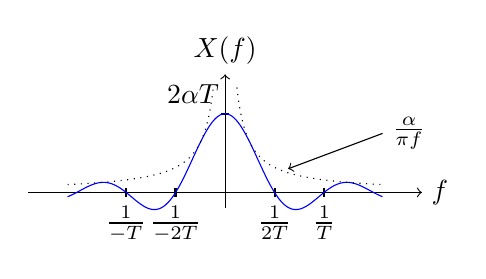
\begin{tikzpicture}[scale=1]
	\draw[->] (-2.5,0) -- (2.5,0) node[right] {$f$};
    \draw[->] (0,-0.2) -- (0,1.5) node[above] {$X(f)$};

\draw[thick] (-1.5pt,1) -- (1.5pt,1) node[above left] {$2\alpha T$};
\draw[thick] (1.26,-1.5pt) -- (1.26,1.5pt) node[below=1mm] {$\frac{1}{T}$};
\draw[thick] (-1.26,-1.5pt) -- (-1.26,1.5pt) node[below=1mm] {$\frac{1}{-T}$};		
\draw[thick] (0.63,-1.5pt) -- (0.63,1.5pt) node[below=1mm] {$\frac{1}{2T}$};
\draw[thick] (-0.63,-1.5pt) -- (-0.63,1.5pt) node[below=1mm] {$\frac{1}{-2T}$};	
		
\draw[color=blue, samples=200, domain=-2:2]   plot (\x,{(sin(5*\x r))/(5*\x)}); 
\draw[dotted, color=black, samples=200, domain=0.15:2]   plot (\x,{1/(5*\x)}); 
\draw[dotted, color=black, samples=200, domain=-2:-0.15]   plot (\x,{-1/(5*\x)}); 

\draw[<-] (0.8,0.3) -- (2,0.75) node[right] {$\frac{\alpha}{\pi f}$};

\end{tikzpicture}
}
\end{tabular}\\ \vspace{6pt}
\textbf{Dreiecksfunktion}
 \begin{equation*}
x(t) = \alpha \cdot \triangle_T(t) = \alpha \cdot \triangle\left( \frac{t}{T}\right)  \qquad
\laplace ~X(f) = \alpha \cdot T \cdot si^2(\pi f T) 
 \end{equation*}
\begin{tabular}{ll}
 \addtolength{\jot}{2mm}
 \parbox{5cm}{
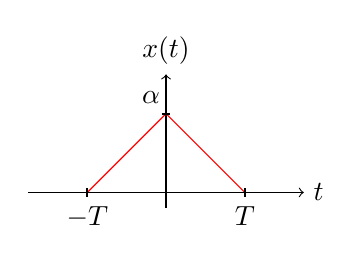
\begin{tikzpicture}[scale=1,
        dot/.style={circle,fill=black,minimum size=3pt,inner sep=0pt,
            outer sep=-1pt}]
	\draw[->] (-1.75,0) -- (1.75,0) node[right] {$t$};
    \draw[->] (0,-0.2) -- (0,1.5) node[above] {$x(t)$};
    	
    \draw[color=red] (-1,0) -- (0,1);
    \draw[color=red] (0,1) -- (1,0);
    
	\draw[thick] (1,-1.5pt) -- (1,1.5pt) node[below=1mm] {$T$};
	\draw[thick] (-1,-1.5pt) -- (-1,1.5pt) node[below=1mm] {$-T$};
	\draw[thick] (-1.5pt,1) -- (1.5pt,1) node[above left] {$\alpha$};	
\end{tikzpicture}
}
 &
 \parbox{5cm}{
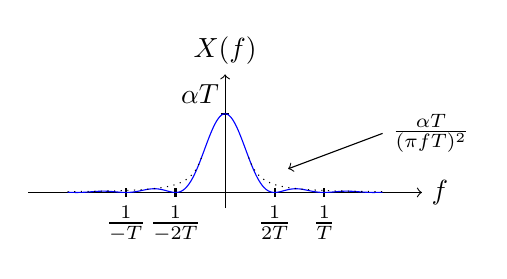
\begin{tikzpicture}[scale=1]
	\draw[->] (-2.5,0) -- (2.5,0) node[right] {$f$};
    \draw[->] (0,-0.2) -- (0,1.5) node[above] {$X(f)$};

\draw[thick] (-1.5pt,1) -- (1.5pt,1) node[above left] {$\alpha T$};
	\draw[thick] (1.26,-1.5pt) -- (1.26,1.5pt) node[below=1mm] {$\frac{1}{T}$};
	\draw[thick] (-1.26,-1.5pt) -- (-1.26,1.5pt) node[below=1mm] {$\frac{1}{-T}$};		
		\draw[thick] (0.63,-1.5pt) -- (0.63,1.5pt) node[below=1mm] {$\frac{1}{2T}$};
	\draw[thick] (-0.63,-1.5pt) -- (-0.63,1.5pt) node[below=1mm] {$\frac{1}{-2T}$};	
		
\draw[color=blue, samples=200, domain=-2:2]   plot (\x,{(sin(5*\x r))/(5*\x)*(sin(5*\x r))/(5*\x)}); 

\draw[dotted, color=black, samples=200, domain=0.30:2]   plot (\x,{1/(5*\x)^2}); 
\draw[dotted, color=black, samples=200, domain=-2:-0.30]   plot (\x,{1/(5*\x)^2}); 

\draw[<-] (0.8,0.3) -- (2,0.75) node[right] {$\frac{\alpha T}{(\pi f T)^2}$};

\end{tikzpicture}
}
\end{tabular}
\\ \vspace{6pt}
\textbf{\SHT -Funktion}
 \begin{equation*}
x(t) = \text{\SHT}_T(t)= \sum_{k \in ~ \mathbb{Z}} \delta(t-kT)  \qquad
\laplace ~X(f) = \frac{1}{T} \text{\SHT}_{\frac{1}{T}}(f)= \sum_{k \in ~ \mathbb{Z}} \delta(f-\frac{k}{T}) 
 \end{equation*}
\begin{tabular}{ll}
 \addtolength{\jot}{2mm}
 \parbox{5cm}{
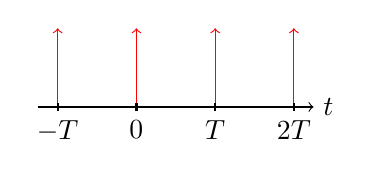
\begin{tikzpicture}[scale=1,
        dot/.style={circle,fill=black,minimum size=3pt,inner sep=0pt,
            outer sep=-1pt}]
	\draw[->] (-1.25,0) -- (2.25,0) node[right] {$t$};
    	
\draw[->, color=red] (-1,0) -- (-1,1);
\draw[->, color=red] (0,0) -- (0,1);
\draw[->, color=red] (1,0) -- (1,1);
\draw[->, color=red] (2,0) -- (2,1);
    
	\draw[thick] (-1,-1.5pt) -- (-1,1.5pt) node[below=1mm] {$-T$};
			\draw[thick] (0,-1.5pt) -- (0,1.5pt) node[below=1mm] {$0$};
		\draw[thick] (1,-1.5pt) -- (1,1.5pt) node[below=1mm] {$T$};
			\draw[thick] (2,-1.5pt) -- (2,1.5pt) node[below=1mm] {$2T$};	
\end{tikzpicture}
}
 &
 \parbox{5cm}{
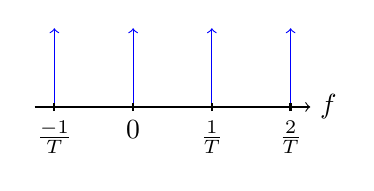
\begin{tikzpicture}[scale=1]
	\draw[->] (-1.25,0) -- (2.25,0) node[right] {$f$};
    	
\draw[->, color=blue] (-1,0) -- (-1,1);
\draw[->, color=blue] (0,0) -- (0,1);
\draw[->, color=blue] (1,0) -- (1,1);
\draw[->, color=blue] (2,0) -- (2,1);
    
	\draw[thick] (-1,-1.5pt) -- (-1,1.5pt) node[below=1mm] {$\frac{-1}{T}$};
			\draw[thick] (0,-1.5pt) -- (0,1.5pt) node[below=1mm] {$0 $};
		\draw[thick] (1,-1.5pt) -- (1,1.5pt) node[below=1mm] {$\frac{1}{T}$};
			\draw[thick] (2,-1.5pt) -- (2,1.5pt) node[below=1mm] {$\frac{2}{T}$};	

\end{tikzpicture}
}
\end{tabular}
\\~
\flushleft
\vfill\columnbreak
\subsection{Operationen mittels Dirac-Impuls}
\begin{tabular}{ll}
 \addtolength{\jot}{2mm}
 \parbox{7cm}{Durch eine Multiplikation im Zeitbereich mit einem Dirac werden alle Funktionswerte, außer an der Stelle des Diracs ausgeblendet. (\textit{Ausblendeigenschaft des Diracs})
\begin{eqnarray*}
r(t) &=& x(t) \cdot \delta(t-t_0) = x(t_0)\\
\delta(t-t_0-t_1) &=& \delta(t-t_0) \ast \delta(t-t_1)
\end{eqnarray*}}&
 \parbox{5cm}{
 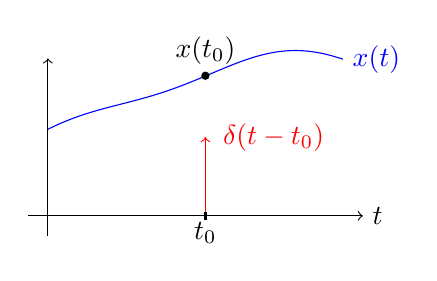
\begin{tikzpicture}[scale=1,domain=0:3.75, dot/.style={circle,fill=black,minimum size=3pt,inner sep=0pt,           outer sep=-1pt}]
	\draw[->] (-0.25,0) -- (4,0) node[right] {$t$};
    \draw[->] (0,-0.25) -- (0,2) node[above] {};

\draw[color=blue, samples=200]   plot (\x,{sin(1/2*\x r)+0.1*cos(2*\x r)+1})   node[right] {$x(t)$}; 
\draw[->, color=red] (2,0) -- (2,1)node[right=1mm] {$\delta(t-t_0)$};
\draw[thick] (2,-1.5pt) -- (2,1.5pt) node[below] {$t_0$};
\node[dot,label=above:$x(t_0)$] at (2,1.78) (int1) {};
\end{tikzpicture}
}
\end{tabular}\\

\begin{tabular}{ll}
 \addtolength{\jot}{2mm}
 \parbox{7cm}{Durch eine Faltung im Zeitbereich wird die Funktion auf die entsprechenden Stellen kopiert (Für Periodische Funktionen kann hier die \SHT -Funktion genutzt werden).
\begin{eqnarray*}
r(t) &=& x(t) \ast \delta(t-t_0) = x(t-t_0)\\
\laplace ~R(f) &=& X(f) \cdot e^{-j2 \pi f t_0}
\end{eqnarray*}}&
 \parbox{5cm}{
 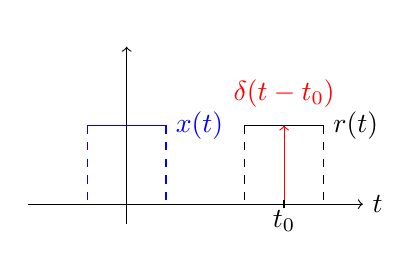
\begin{tikzpicture}[scale=1,domain=0:3.75, dot/.style={circle,fill=black,minimum size=3pt,inner sep=0pt,           outer sep=-1pt}]
	\draw[->] (-1.25,0) -- (3,0) node[right] {$t$};
    \draw[->] (0,-0.25) -- (0,2) node[above] {};

\draw[color=blue] (-0.5,1) -- (0.5,1)node[right] {$x(t)$};
\draw[dashed, color=blue] (-0.5,1) -- (-0.5,0);
\draw[dashed, color=blue] (0.5,1) -- (0.5,0);
	
\draw[->, color=red] (2,0) -- (2,1)node[above=1mm] {$\delta(t-t_0)$};

\draw[thick] (2,-1.5pt) -- (2,1.5pt) node[below] {$t_0$};

\draw[color=black] (1.5,1) -- (2.5,1)node[right] {$r(t)$};
\draw[dashed, color=black] (1.5,1) -- (1.5,0);
\draw[dashed, color=black] (2.5,1) -- (2.5,0);
\end{tikzpicture}
}
\end{tabular}
\subsection{Elementare Operationen für Funktionen}
\textbf{Elementare Operationen} für Funktionen sind folgende:\\
\begin{tabular}{ll}
 \addtolength{\jot}{2mm}
 \parbox{7cm}{
  \centering
zeitliche Verschiebung der Funktionen
 \begin{eqnarray*}
rot: x_1(t) &=& \alpha \cdot \xi(t-t_1)\\
blau: x_2(t) &=& \alpha \cdot \xi(t+t_2)
 \end{eqnarray*}}
 &
 \parbox{5cm}{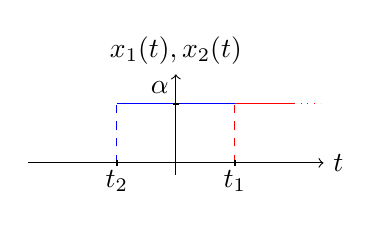
\begin{tikzpicture}[scale=0.75,
        dot/.style={circle,fill=black,minimum size=3pt,inner sep=0pt,
            outer sep=-1pt}]
	\draw[->] (-2.5,0) -- (2.5,0) node[right] {$t$};
    \draw[->] (0,-0.2) -- (0,1.5) node[above] {$x_1(t), x_2(t)$};
	
	\draw[dashed, color=blue] (-1,0) -- (-1,1);
	\draw[color=blue] (-1,1) -- (2,1);
	
    \draw[dashed, color=red] (1,0) -- (1,1);
	\draw[color=red] (1,1) -- (2,1);
	\draw[dotted, color=red] (2,1) -- (2.45,1);
			
	\draw[thick] (-1,-1.5pt) -- (-1,1.5pt) node[below] {$t_2$};		
	\draw[thick] (1,-1.5pt) -- (1,1.5pt) node[below] {$t_1$};	
	\draw[thick] (-1.5pt,1) -- (1.5pt,1) node[above left] {$\alpha$};	
\end{tikzpicture}
}
\end{tabular}
\begin{tabular}{ll}
 \addtolength{\jot}{2mm}
 \parbox{7cm}{
  \centering
Spiegelung
 \begin{eqnarray*}
x(t) &=& \alpha \cdot \xi(t_0-t)\\
 \end{eqnarray*}}
 &
 \parbox{5cm}{\begin{tikzpicture}[scale=0.75,
        dot/.style={circle,fill=black,minimum size=3pt,inner sep=0pt,
            outer sep=-1pt}]
	\draw[->] (-2.5,0) -- (2.5,0) node[right] {$t$};
    \draw[->] (0,-0.2) -- (0,1.5) node[above] {$x(t)$};
	
    \draw[dashed, color=red] (1,0) -- (1,1);
	\draw[color=red] (1,1) -- (-2,1);
	\draw[dotted, color=red] (-2,1) -- (-2.45,1);
	
	\draw[thick] (1,-1.5pt) -- (1,1.5pt) node[below] {$t_0$};	
	\draw[thick] (-1.5pt,1) -- (1.5pt,1) node[above left] {$\alpha$};		
\end{tikzpicture}
}
\end{tabular}
\begin{tabular}{ll}
 \addtolength{\jot}{2mm}
 \parbox{7cm}{
  \centering
Zeitliche Skalierung
 \begin{eqnarray*}
blau: x_1(t) &=& sin(t)\\
rot: x_2(t) &=& sin(2 \cdot t)\\
sin( \alpha \cdot t) &=& \begin{cases} \alpha < 1 &\text{,Dehung}\\
 \alpha > 1 &\text{,Stauchung} \end{cases}
 \end{eqnarray*}}
 &
 \parbox{5cm}{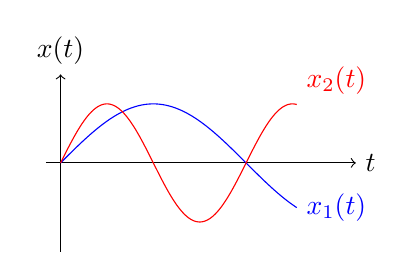
\begin{tikzpicture}[scale=0.75,
        dot/.style={circle,fill=black,minimum size=3pt,inner sep=0pt,
            outer sep=-1pt},
        domain=0:4]
	\draw[->] (-0.25,0) -- (5,0) node[right] {$t$};
    \draw[->] (0,-1.5) -- (0,1.5) node[above] {$x(t)$};
	
\draw[color=blue, samples=200]   plot (\x,{sin(\x r)})   node[right] {$x_1(t)$}; 
\draw[color=red, samples=200]   plot (\x,{sin(2*\x r)})   node[above right] {$x_2(t)$}; 
\end{tikzpicture}
}
\end{tabular}
\begin{tabular}{ll}
 \addtolength{\jot}{2mm}
 \parbox{7cm}{
\flushleft
\textbf{Beispiel} einer Rechteckfunktion
 \begin{eqnarray*}
x(t) &=& rect(2t-4)\\
&=& rect(2(t-2))
 \end{eqnarray*}}
 &
 \parbox{5cm}{\begin{tikzpicture}[scale=1,
        dot/.style={circle,fill=black,minimum size=3pt,inner sep=0pt,
            outer sep=-1pt}]
	\draw[->] (-0.25,0) -- (4,0) node[right] {$t$};
    \draw[->] (0,-0.2) -- (0,1.5) node[above] {$x(t)$};
	
    \draw[dashed, color=red] (1,0) -- (1,1);
	\draw[color=red] (1,1) -- (3,1);
	\draw[dashed, color=red] (3,0) -- (3,1);
	\draw[dotted] (0,1)--(1,1);
	
	\draw (3,-0.1) -- (3,0.1); 
	\draw (2,-0.1) -- (2,0.1); 
	\draw (1,-0.1) -- (1,0.1);
	\draw (-0.1,1) -- (0.1,1);  		
	\node[label=below:$2.5$] at (3,0) (int1) {};
	\node[label=below:$2$] at (2,0) (int1) {};
	\node[label=below:$1.5$] at (1,0) (int1) {};	
	\node[label=above left:$1$] at (0,1) (int1) {};
\end{tikzpicture}
}
\end{tabular}\\
~
\vfill\columnbreak
\subsection{Faltung}
\begin{tabular}{ll}
 \addtolength{\jot}{2mm}
 \parbox{7cm}{Faltung \label{Falt} ist eine rückwärts gerichtete Gewichtung mit einer Gewichtungsfunktion $c(t)$ aller vorherigen Eingangssignale $s(t)$.\\
\begin{eqnarray*}
r(t) &=&  c(t) \ast s(t)\\
&=&  \int_0^{t} c(t - \tau ) ~ s( \tau)~ d \tau \\
&=& \int_0^{t} s(t -  \tau) ~ c(\tau ) ~ d \tau \\
&=& \int_0^{t} s(-(\tau - t ))~ c(\tau )  ~ d \tau
\end{eqnarray*}
Das Ausgangssignal $r(t_0)$ setzt sich somit aus der zeitlich verschobenen und gespiegelten Gewichtsfunktion $c(t_0 - \tau )$ und dem Eingangssignal $s(t)$ zusammen.
 }&
 \parbox{5cm}{
 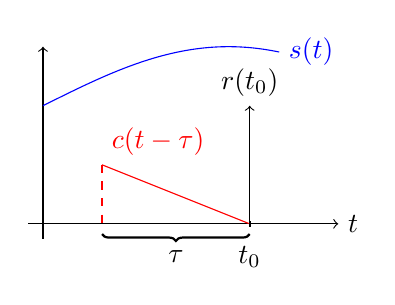
\begin{tikzpicture}[scale=0.75,
        dot/.style={circle,fill=black,minimum size=3pt,inner sep=0pt,
            outer sep=-1pt},
        domain=0:4]
	\draw[->] (-0.25,0) -- (5,0) node[right] {$t$};
    \draw[->] (0,-0.25) -- (0,3) node[above] {};
	
\draw[color=blue, samples=200]   plot (\x,{sin(1/2*\x r)+2})   node[right] {$s(t)$}; 

\draw[color=red] (3.5,0) -- (1,1)node [above right] {$c(t- \tau)$};;
\draw[dashed, color=red] (1,1) -- (1,0) ;

\draw[thick] (3.5,-1.5pt) -- (3.5,1.5pt) node[below=2mm] {$t_0$};
\draw[->, color=black] (3.5,0) -- (3.5,2)node [above] {$r(t_0)$}; 

\draw[thick, decoration={brace, mirror, raise=0.5}, decorate] (1,-0.15) -- (3.5,-0.15) node[pos=0.5,anchor=north,yshift=-0.1cm]{$\tau$};
\end{tikzpicture}
}
\end{tabular}\\
\vspace{6pt}
\begin{tabular}{ll}
 \addtolength{\jot}{2mm}
 \parbox{6cm}{
 Es gelten folgende Faltungsregeln:
 \begin{eqnarray*}
x(t) \ast h(t) &=& h(t) \ast x(t)\\
(x(t) \ast h(t)) \ast g(t) &=&  x(t) \ast (h(t) \ast g(t))\\
rect(t-t_1) \ast rect(t-t_2)&=& \triangle(t-1-t_1-t_2)
 \end{eqnarray*}}
 &
 \addtolength{\jot}{2mm}
 \parbox{5cm}{\begin{eqnarray*}
(x_1(t) + x_2(t)) \ast h(t) &=&  h(t) \ast x_1(t) + h(t) \ast x_2(t)\\
x(t) \ast \delta(t) &=& x(t)\\
x(t) \ast \delta(t-t_0) &=& x(t-t_0)
  \end{eqnarray*}}
\end{tabular}
\begin{eqnarray*}
\alpha \cdot \beta \cdot \delta(t-t_0) \ast \delta(t-t_1) &=& \alpha \cdot \delta(t-t_0) \ast \beta  \cdot \delta(t-t_1)
\end{eqnarray*}\\~
\begin{tabular}{ll}
 \addtolength{\jot}{2mm}
 \parbox{7cm}{
 \textbf{Beispiel:}\\
 \centering
 Ein Rechteck mit einem Rechteck gefaltet: \\
 \vspace{6pt} 
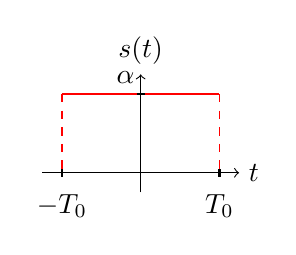
\begin{tikzpicture}[scale=1,
        dot/.style={circle,fill=black,minimum size=3pt,inner sep=0pt,
            outer sep=-1pt},domain=0:4]
            
\draw[->] (-1.25,0) -- (1.25,0) node[right] {$t$};
\draw[->] (0,-0.25) -- (0,1.25) node[above] {$s(t)$};

\draw[dashed, color=red] (-1,1) -- (-1,0) ;	
\draw[color=red] (-1,1) -- (1,1);
\draw[dashed, color=red] (1,1) -- (1,0) ;

\draw[thick] (-1,-1.5pt) -- (-1,1.5pt) node[below=2mm] {$-T_0$};
\draw[thick] (1,-1.5pt) -- (1,1.5pt) node[below=2mm] {$T_0$};
\draw[thick] (-1.5pt,1) -- (1.5pt,1) node[above left] {$\alpha$};
\end{tikzpicture}
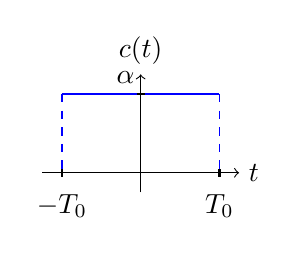
\begin{tikzpicture}[scale=1,
        dot/.style={circle,fill=black,minimum size=3pt,inner sep=0pt,
            outer sep=-1pt},domain=0:4]
            
\draw[->] (-1.25,0) -- (1.25,0) node[right] {$t$};
\draw[->] (0,-0.25) -- (0,1.25) node[above] {$c(t)$};

\draw[dashed, color=blue] (-1,1) -- (-1,0) ;	
\draw[color=blue] (-1,1) -- (1,1);
\draw[dashed, color=blue] (1,1) -- (1,0) ;

\draw[thick] (-1,-1.5pt) -- (-1,1.5pt) node[below=2mm] {$-T_0$};
\draw[thick] (1,-1.5pt) -- (1,1.5pt) node[below=2mm] {$T_0$};
\draw[thick] (-1.5pt,1) -- (1.5pt,1) node[above left] {$\alpha$};
\end{tikzpicture}}
 &
 \parbox{5cm}{
 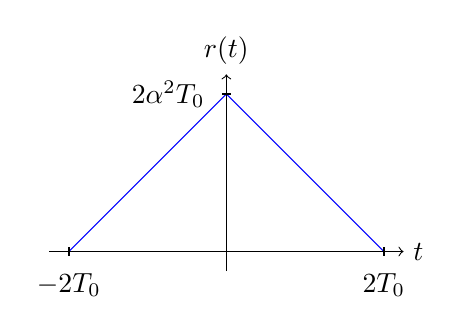
\begin{tikzpicture}[scale=1,
        dot/.style={circle,fill=black,minimum size=3pt,inner sep=0pt,
            outer sep=-1pt},domain=0:4]
\draw[->] (-2.25,0) -- (2.25,0) node[right] {$t$};
\draw[->] (0,-0.25) -- (0,2.25) node[above] {$r(t)$};
	
\draw[color=blue] (-2,0) -- (0,2);;
\draw[color=blue] (0,2) -- (2,0);

\draw[thick] (2,-1.5pt) -- (2,1.5pt) node[below=2mm] {$2T_0$};
\draw[thick] (-1.5pt,2) -- (1.5pt,2) node[left=2mm] {$2 \alpha^2 T_0$};   
\draw[thick] (-2,-1.5pt) -- (-2,1.5pt) node[below=2mm] {$-2T_0$};          
\end{tikzpicture}
}
\end{tabular}\\
Beide Funktionen sind definiert nach:\\
\begin{equation*}
s(t) = c(t) = \begin{cases} \alpha &\text{\qquad $-T_0 <$ t $< T_0$}\\
						0 &\text{\qquad sonst}
						\end{cases}
\end{equation*}
Für die Faltung daraus ergibt sich:\\
\begin{eqnarray*}
r(t) = s(t) \ast c(t) &=&  \int_{-\infty}^\infty s( \tau) c(t - \tau )  d \tau \\
&=&  \begin{cases} \displaystyle \int_{-T_0}^{t+T_0} \alpha \cdot \alpha ~d \tau = \alpha^2(t+2T_0)		&\text{\qquad $-2T_0 <$ t $< 0$}\\[1em]
					\displaystyle \int_{t-T_0}^{T_0} \alpha \cdot \alpha ~d \tau = \alpha^2(2T_0-t)		&\text{\qquad $0 <$ t $< 2T_0$}
	\end{cases}\\
\end{eqnarray*}\\~
\flushleft
\subsection{Lineare Systeme}
\begin{tabular}{ll}
 \addtolength{\jot}{2mm}
 \parbox{7cm}{Allgemein wird ein Übertragungskanal auch System bezeichnet. Ein System faltet ein Eingangssignal \textit{s(t)} mit einer Gewichtsfunktion \textit{c(t)}, dem sogenannten \textbf{Kern} des Systems. Diese Faltung wird in Abschnitt \ref{Falt} erläutert. Für Lineare Systeme gelten folgende Eigenschaften die zu beweisen sind:
\begin{equation*}
r(t) = \int_\mathbb{R} s(u) \cdot k(t;u)~ du
\end{equation*} 
 }
 &
 \parbox{5cm}{
 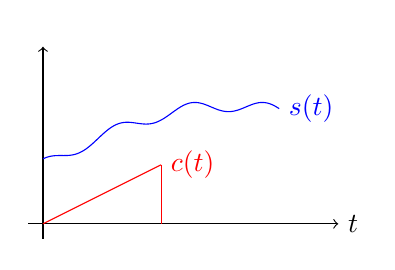
\begin{tikzpicture}[scale=0.75,
        dot/.style={circle,fill=black,minimum size=3pt,inner sep=0pt,
            outer sep=-1pt},
        domain=0:4]
	\draw[->] (-0.25,0) -- (5,0) node[right] {$t$};
    \draw[->] (0,-0.25) -- (0,3) node[above] {};
	
\draw[color=blue, samples=200]   plot (\x,{sin(1/2*\x r)+0.1*cos(5*\x r)+1})   node[right] {$s(t)$}; 
\draw[color=red] (0,0) -- (2,1)node [right] {$c(t)$};;
\draw[color=red] (2,1) -- (2,0) ;
\end{tikzpicture}
}
\end{tabular}\\
\vspace{6pt}
\begin{tabular}{ll}
 \addtolength{\jot}{2mm}
 \parbox{7cm}{
  \centering
\textbf{Linearität}\\
Ein Eingangssignal kann aus mehreren gewichteten Signalen bestehen und ein Ausgangssignal erzeugen
 \begin{eqnarray*}
\mathcal{H}(\alpha s_1(t) + \beta s_2(t)) &=& \alpha \mathcal{H}(s_1(t)) + \beta \mathcal{H}(s_2(t))\\
r(t) &=& r_1(t) + r_2(t)
 \end{eqnarray*}}
 &
 \parbox{5cm}{
 \begin{tikzpicture}[node distance=2.5cm,auto,>=latex']
	\node [int] (a) {System $\mathcal{H}$};
    \node (b) [left of=a,node distance=2cm, coordinate] {a};
    \node [coordinate] (end) [right of=a, node distance=2cm]{};
    \path[->] (b) edge node {$s(t)$} (a);
    \draw[->] (a) edge node {$r(t)$} (end) ;
\end{tikzpicture}
}
\end{tabular}\\
\vspace{6pt}
\textbf{1. Beispiel:} \qquad $r(t) = s(t-1)\cdot cos(\omega t)$ \quad $\omega = const.$
\begin{eqnarray*} \mathcal{H}(\alpha r_1(t) + \beta r_2(t)) &=& 
	\alpha \cdot \underbrace{s_1(t-1)\cdot cos(\omega t)}_{r_1(t)} + \beta \cdot \underbrace{s_2(t-1)\cdot cos(\omega t)}_{r_2(t)}\\
&=& \alpha \cdot \mathcal{H}(r_1(t)) + \beta \cdot \mathcal{H}(r_2(t))\\
&\Rightarrow& \text{lineares System}\\
\end{eqnarray*}
\textbf{2. Beispiel:} \qquad $r(t) = s(t) \cdot \frac{\delta s(t)}{\delta t}$ \qquad für z.B. $s(t) = t^2$ und $\alpha = 2$
\begin{eqnarray*} \mathcal{H}(\alpha s(t) = \mathcal{H}(2t^2) &=& 2t^2 \cdot 4t = 8t^3\\
 \alpha  \mathcal{H}(s(t) = 2 \cdot \mathcal{H}(t^2) &=& 2(t^2 \cdot 2t) = 4t^3\\
&\Rightarrow& \text{nichtlineares System} 
\end{eqnarray*}
\vspace{6pt}
\begin{tabular}{ll}
 \addtolength{\jot}{2mm}
 \parbox{7cm}{
  \centering
\textbf{Kern}\\
\flushleft
Jede lineare Abbildung hat einen Kern, wenn das System nicht linear ist existiert kein Kern. Bei linear zeitinvarianten Systemen (LTI) ist der Kern nicht zeitabhängig und somit konstant.
 \begin{eqnarray*}
k(t; u) &=& \mathcal{H}(\delta(t-u))\\
\text{LTI-Systemen:} &\Rightarrow& k(t,t-\tau) = c(\tau)
 \end{eqnarray*}}
 &
 \parbox{5cm}{ 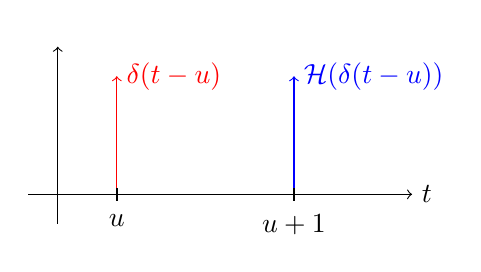
\begin{tikzpicture}[scale=1.5,
        dot/.style={circle,fill=black,minimum size=3pt,inner sep=0pt,
            outer sep=-1pt}]
	\draw[->] (-0.25,0) -- (3,0) node[right] {$t$};
    \draw[->] (0,-0.25) -- (0,1.25) node[above] {};
	
\draw[->, color=red] (0.5,0) -- (0.5,1)node [right] {$\delta(t-u)$};
\draw[thick] (0.5,-1.5pt) -- (0.5,1.5pt) node[below=2mm] {$u$};
\draw[->, color=blue] (2,0) -- (2,1)node [right] {$\mathcal{H}(\delta(t-u))$};
\draw[thick] (2,-1.5pt) -- (2,1.5pt) node[below=2mm] {$u+1$};
\end{tikzpicture}\\
\centering
Graph zu Bsp. 3
}
\end{tabular}\\
\begin{tabular}{ll}
 \addtolength{\jot}{2mm}
 \parbox{7cm}{
  \centering
\textbf{Zeitvarianz und Zeitinvarianz}\\
Die Zeitvarianz eines Systems kann durch den Kern des Systems bestimmt werden. Ist der Kern des Systems neben dem Dirac-Impuls von einer weiteren Zeitabhängigen Variable abhängig, ist das System zeitvariant.
 \begin{eqnarray*}
r(t-t_0) &=& \mathcal{H}(s(t-t_0))
 \end{eqnarray*}}
 &
 \parbox{5cm}{ 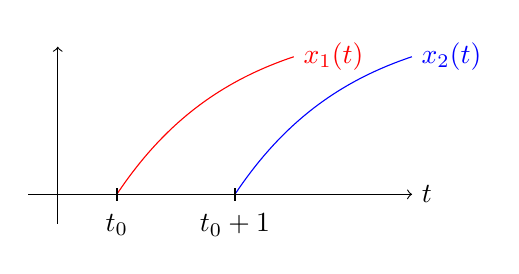
\begin{tikzpicture}[scale=1.5,
        dot/.style={circle,fill=black,minimum size=3pt,inner sep=0pt,
            outer sep=-1pt}]
	\draw[->] (-0.25,0) -- (3,0) node[right] {$t$};
    \draw[->] (0,-0.25) -- (0,1.25) node[above] {};
	
\draw[color=red, samples=150, domain=0:1.5, xshift=0.5cm]   plot (\x,{1.5*(1-exp(-1*\x))})   node[right] {$x_1(t)$}; 
\draw[thick] (0.5,-1.5pt) -- (0.5,1.5pt) node[below=2mm] {$t_0$};
\draw[color=blue, samples=150, domain=0:1.5, xshift=1.5cm]   plot (\x,{1.5*(1-exp(-1*\x))})   node[right] {$x_2(t)$}; 
\draw[thick] (1.5,-1.5pt) -- (1.5,1.5pt) node[below=2mm] {$t_0+1$};
\end{tikzpicture}\\
\centering
Zeitinvariant: Egal welcher Startpunkt, Funktion ist immer gleich
}
\end{tabular}\\~
\vfill\columnbreak
\vspace{6pt}
\textbf{1. Beispiel:} \qquad $r(t) = s(t-1)\cdot cos(\omega t)$ \quad $\omega = const.$
\begin{eqnarray*} 
k(t; u) &=& \mathcal{H}(\delta(t-u) =\underbrace{\delta(t-u-1) \cdot cos(\omega t)} _{\text{Kern}} \qquad \Rightarrow \text{Zeitvariant durch $cos( \omega t)$}
\end{eqnarray*}
\textbf{2. Beispiel:} \qquad $r(t) = s(t) \cdot t^2$ 
\begin{eqnarray*} 
k(t; u) &=& \mathcal{H}(\delta(t-u)) = \underbrace{\delta(t-u) \cdot t^2} _{\text{Kern}} \qquad \Rightarrow \text{Zeitvariant durch $t^2$}
\end{eqnarray*}
\textbf{3. Beispiel:} \qquad $r(t) = s(t-1)$
\begin{eqnarray*} 
k(t; u) &=& \mathcal{H}(\delta(t-u)) =\underbrace{\delta(t-u-1)} _{\text{Kern}} \qquad \Rightarrow \text{Zeitinvariant(LTI-System)}
\end{eqnarray*}
\vspace{6pt}
\begin{tabular}{ll}
 \addtolength{\jot}{2mm}
 \parbox{7cm}{
  \centering
\textbf{Gedächtnis und Kausalität}\\
\flushleft
Ein System ist nur Kausal, wenn es auf Eingangswerte der Vergangenheit zurückgreift. Das Ausgangssignal eines gedächtnisloses System hängt zu jedem Zeitpunkt $t_0$ nur von dem Eingangssignal $s(t_0)$ zum selben Zeitpunkt ab.
\begin{eqnarray*}
r(t_0) &=& \mathcal{H}(s(t)) \qquad \text{für}~ t \leqslant t_0 
\end{eqnarray*}}
 &
 \parbox{7cm}{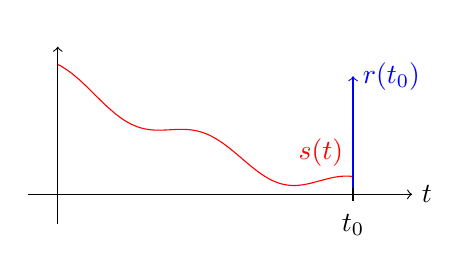
\begin{tikzpicture}[scale=1.5,
        dot/.style={circle,fill=black,minimum size=3pt,inner sep=0pt,
            outer sep=-1pt}]
	\draw[->] (-0.25,0) -- (3,0) node[right] {$t$};
    \draw[->] (0,-0.25) -- (0,1.25) node[above] {};
	
\draw[color=red, samples=150, domain=0:2.5, xshift=0.0cm]   plot (\x,{sin(-1/2*\x r)+0.1*cos(5*\x r)+1})   node[above left] {$s(t)$}; 
\draw[->, color=blue] (2.5,0) -- (2.5,1)node [right] {$r(t_0)$}; 
\draw[thick] (2.5,-1.5pt) -- (2.5,1.5pt) node[below=2mm] {$t_0$};
\end{tikzpicture}
}
\end{tabular}
\textbf{Beispiel:} \qquad $r(t) = \int^t_0 s(t- \tau) \left[ c( \tau) \right]^2 d \tau $
\begin{eqnarray*} 
k(t; u) &=& \mathcal{H}(\delta(t-u)) = \int^t_0 \delta(t-u- \tau) \left[ c( \tau) \right]^2 d \tau \\
&=& \int^\infty_\infty \delta(t-u- \tau) \left[ c( \tau) \right]^2 \cdot \underbrace{\left[  \xi( \tau) - \xi (t- \tau) \right]}_{Rechteck} d \tau \\
&=&  \left[ c(t - u) \right]^2\left[  \xi(t - u) - \xi (t- t - u) \right]  \\
&=&  \underbrace{\left[ c(t - u) \right]^2\left[  \xi(u) - \xi (u-t) \right] )} _{\text{Kern}} \\
\end{eqnarray*}
\begin{tabular}{ll}
 \addtolength{\jot}{2mm}
 \parbox{6cm}{
 Die Rechteckfunktion aus den Einheitsprungen wird genutzt um alles außerhalb $0< \tau < t$ auszublenden. Dazu kommt noch die Ausblendeigenschaft des Diracs an der Stelle $(t-u) = \tau$.
}
 &
 \parbox{7cm}{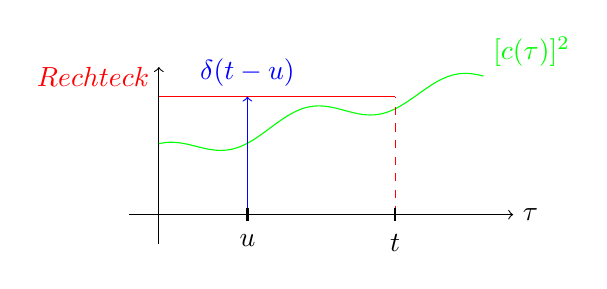
\begin{tikzpicture}[scale=1.5,
        dot/.style={circle,fill=black,minimum size=3pt,inner sep=0pt,
            outer sep=-1pt}]
	\draw[->] (-0.25,0) -- (3,0) node[right] {$\tau$};
    \draw[->] (0,-0.25) -- (0,1.25) node[above] {};
	
\draw[color=green, samples=150, domain=0:2.75, xshift=0.0cm]   plot (\x,{sin(1/4*\x r)+0.1*cos(5*\x r)+0.5})   node[above right] {$[c(\tau)]^2$};
 
\draw[color=red] (2,1) -- (0,1)node [above left] {$Rechteck$};
\draw[dashed, color=red] (2,0) -- (2,1);
\draw[thick] (2,-1.5pt) -- (2,1.5pt) node[below=2mm] {$t$};
	
\draw[->, color=blue] (0.75,0) -- (0.75,1)node [above] {$\delta(t-u)$}; 
\draw[thick] (0.75,-1.5pt) -- (0.75,1.5pt) node[below=2mm] {$u$};

\end{tikzpicture}
}
\end{tabular}
\vspace{6pt} \\
$\Rightarrow$ Das System ist zeitvariant, da es zusätzlich von $\xi(u-t)$ abhängt.Zudem benötigt man für:
\begin{equation*}
r(-1) = \int^{-1}_0 s(-1- \tau) \left[ c( \tau) \right]^2 d \tau = - \int^0_{-1} s(-1- \tau) \left[ c( \tau) \right]^2 d \tau
\end{equation*}
 
den Wert an der Stelle $s(0)$. Dieser liegt in der Zukunft $\Rightarrow$ Akausal.\\
Das System ist für $c( \tau) = 0 ~ \forall ~ \tau < 0$ kausal. Zudem ist es Gedächtnisbehaftet, da es auf Werte in der Vergangenheit zurückgreift, bei $r(2)$ auf alle Werte von $s(0)$ bis $s(2)$.
\begin{equation*}
r(2) = \int^{2}_0 s(2 - \tau) \left[ c( \tau) \right]^2 d \tau
\end{equation*}
\subsection{Fouriereihe zur Darstellung periodischer Signale}
\begin{tabular}{ll}
 \addtolength{\jot}{2mm}
 \parbox{5cm}{Allgemein gilt für die Fouriereihe im komplexen Fall mit dem \textbf{Fouriekoeffizenz} $c_n$ dieser im allgemeinen Fall auch bestimmt werden kann. Die Bestimmung des Koeffizenten kann auch mittels \SHT -Funktion erfolgen. Die Fouriereihe kann auch in Realteil und Imaginärteil aufgeteilt werden:}
 &
 \parbox{5cm}{\begin{eqnarray*}
r(t) &=& \sum^\infty_{n = - \infty} c_n \cdot e^{j2\pi n \frac{t}{T}}\\
c_n &=&  \frac{1}{T} \int^T_0 r(t) \cdot  e^{-j2\pi n \frac{t}{T}} dt
\end{eqnarray*}
}
\end{tabular}\\
\begin{equation*}
r(t) = \frac{a_0}{2} + \sum^\infty_{n = 1} a_n \cdot cos \left( 2\pi n \frac{t}{T}\right)  +  \sum^\infty_{n = 1} b_n  \cdot sin\left(2\pi n \frac{t}{T}\right) 
\end{equation*}\\
\begin{tabular}{ll}
 \addtolength{\jot}{2mm}
 \parbox{5cm}{Für die reellen und imaginären Koeffizienten gelten dann die Eigenschaften:\\
\begin{align*}
a_n &= c_n + c_{-n} &n=0,1,2,... \\
b_n &= j(c_n + c_{-n}) &n=1,2,... \\
a_0 &= c_0 + c_0 = 2c_0 &~ \\
\end{align*} 
 }
 &
 \parbox{5cm}{
 \begin{eqnarray*}
a_n &=& \frac{2}{T} \int^T_0 r(t) \cdot  cos \left(2\pi n \frac{t}{T}\right)  dt\\
b_n &=&  \frac{2}{T} \int^T_0 r(t) \cdot  sin \left(2\pi n \frac{t}{T}\right)  dt
\end{eqnarray*}
}
\end{tabular}\\


\begin{tabular}{ll}
 \addtolength{\jot}{2mm}
 \parbox{5cm}{
 \textbf{Beispiel:}\\
\begin{eqnarray*}
 r(t) &=& t \text{\qquad für 0 $<$ t $<$ 1} \\
 r(0) &=& \frac{1}{2} \\
 T &=& 1
\end{eqnarray*}}
 &
 \parbox{5cm}{
 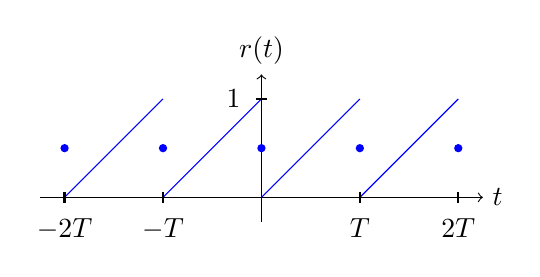
\begin{tikzpicture}[scale=1.25,
        dot/.style={circle,fill=blue,minimum size=3pt,inner sep=0pt,
            outer sep=-1pt},domain=0:4]
\draw[->] (-2.25,0) -- (2.25,0) node[right] {$t$};
\draw[->] (0,-0.25) -- (0,1.25) node[above] {$r(t)$};

\draw[color=blue] (-2,0) -- (-1,1);
\draw[color=blue] (-1,0) -- (0,1);	
\draw[color=blue] (0,0) -- (1,1);
\draw[color=blue] (1,0) -- (2,1);

\draw[thick] (-2,-1.5pt) -- (-2,1.5pt) node[below=2mm] {$-2T$};
\draw[thick] (-1,-1.5pt) -- (-1,1.5pt) node[below=2mm] {$-T$};
\draw[thick] (1,-1.5pt) -- (1,1.5pt) node[below=2mm] {$T$};
\draw[thick] (-1.5pt,1) -- (1.5pt,1) node[left=2mm] {$1$};   
\draw[thick] (2,-1.5pt) -- (2,1.5pt) node[below=2mm] {$2T$}; 

\node[dot] at (-2,0.5) (int1) {}; 
\node[dot] at (-1,0.5) (int1) {};  
\node[dot] at (0,0.5) (int1) {}; 
\node[dot] at (1,0.5) (int1) {};   
\node[dot] at (2,0.5) (int1) {};         
\end{tikzpicture}}
\end{tabular}
\\~
Finden der komplexen Koeffizienten $c_k$ dieser Fourierreihe mittels der Definition:
\begin{eqnarray*}
c_k &=& \frac{1}{1} \int_0^1 e^{-j2 \pi k \frac{t}{1}} \cdot t ~ dt = \int_0^1 e^{-j2 \pi kt} \cdot t ~ dt
\end{eqnarray*}
Substitution mit \qquad $u=t \quad u' = 1 \qquad \qquad v' = e^{-j2 \pi kt} \quad v = \frac{1}{-j2 \pi k} \cdot e^{-j2 \pi kt} $
\begin{eqnarray*}
c_k &=&  \underbrace{\left[ \frac{-t}{j2 \pi k}e^{-j2 \pi kt} \right]^1_0}_{u \cdot v} -  \underbrace{\int^1_0 \frac{-1}{j2 \pi k}  e^{-j2 \pi kt} ~ dt}_{u' \cdot v}
 = \frac{-1}{j2 \pi k} e^{-j2 \pi k} + \left( \frac{1}{j2 \pi k}\right)\left[\frac{1}{-j2 \pi k} e^{-j2 \pi kt} 
\right]^1_0\\
&=& \frac{-1}{j2 \pi k} \underbrace{e^{-j2 \pi k}}_{=1} + \underbrace{\left( \frac{1}{j2 \pi k}\right)^2 \underbrace{e^{-j2 \pi kt}}_{=e^{-j2 \pi k}-1} \bigg\vert^1_0 }_{= 0} = \frac{-1}{j2 \pi k} = \frac{j}{2 \pi k}\\
&\Rightarrow& c_1 , c_2 , ...=\frac{j}{2 \pi k} \qquad k \ne 0 \qquad \qquad \Rightarrow \vert c_k \vert = \frac{1}{2 \pi} \cdot \frac{1}{\vert k \vert}\qquad k \ne 0\\
\text{für k = 0:} \quad &\Rightarrow& c_0 = \frac{1}{1} \int^1_0 t ~ dt = \frac{1}{2}t^2 \bigg\vert^1_0 = \frac{1}{2}  \qquad \qquad k = 0 \qquad ( Da~e^{j2 \pi \cdot 0 \cdot t} = 1 \quad ,bei~t = 0)
\end{eqnarray*}\\
Es gilt dann für die Fourierreihe durch einsetzen der Koeffizienten $c_0$ und $c_k$:
\begin{eqnarray*}
&\Rightarrow& r(t) = \frac{1}{2} + \sum_{k \neq 0}\frac{j}{2 \pi k} e^{j2 \pi kt}
\end{eqnarray*}
\subsection{\SHT-Funktion zur Darstellung periodischer Signale}

\begin{tabular}{ll}
 \addtolength{\jot}{2mm}
 \parbox{6cm}{
Durch die Faltung einer nichtperiodischen Funktion (Grundfunktion) $x_0(t)$ mit der Kammfunktion oder \SHT -Funktion im Zeitbereich, kann die nichtperiodische Funktionen eine Periodizität erlangen. Die Grundfunktion wird sozusagen an die stellen des Diracs kopiert (siehe schwarz). Die entstandene Funktion heißt nun $x(t)$.
} &
 \parbox{5cm}{
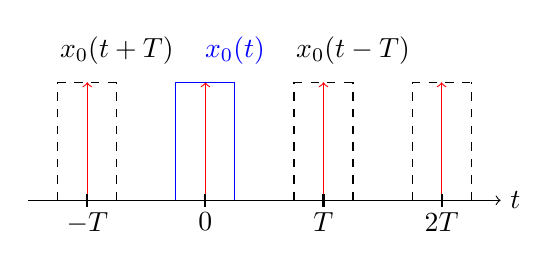
\begin{tikzpicture}[scale=1.5,
        dot/.style={circle,fill=black,minimum size=3pt,inner sep=0pt,
            outer sep=-1pt}]
	\draw[->] (-1.5,0) -- (2.5,0) node[right] {$t$};
    	
\draw[->, color=red] (-1,0) -- (-1,1);
\draw[->, color=red] (0,0) -- (0,1);
\draw[->, color=red] (1,0) -- (1,1);
\draw[->, color=red] (2,0) -- (2,1);

\draw[color=blue] (-0.25,0) -- (-0.25,1);
\draw[color=blue] (-0.25,1) -- (0.25,1) node[above=1mm] {$x_0(t)$};
\draw[color=blue] (0.25,0) -- (0.25,1);

\draw[color=black, dashed] (-1.25,0) -- (-1.25,1);
\draw[color=black, dashed] (-1.25,1) -- (-0.75,1) node[above=1mm] {$x_0(t+T)$};
\draw[color=black, dashed] (-0.75,0) -- (-0.75,1);

\draw[color=black, dashed] (0.75,0) -- (0.75,1);
\draw[color=black, dashed] (0.75,1) -- (1.25,1) node[above=1mm] {$x_0(t-T)$};
\draw[color=black, dashed] (1.25,0) -- (1.25,1);

\draw[color=black, dashed] (1.75,0) -- (1.75,1);
\draw[color=black, dashed] (1.75,1) -- (2.25,1);
\draw[color=black, dashed] (2.25,0) -- (2.25,1);
    
\draw[thick] (-1,-1.5pt) -- (-1,1.5pt) node[below=1mm] {$-T$};
\draw[thick] (0,-1.5pt) -- (0,1.5pt) node[below=1mm] {$0$};
\draw[thick] (1,-1.5pt) -- (1,1.5pt) node[below=1mm] {$T$};
\draw[thick] (2,-1.5pt) -- (2,1.5pt) node[below=1mm] {$2T$};	
\end{tikzpicture}
}
\end{tabular}
\begin{eqnarray*}
x(t) &=& \sum_{k~\in~\mathbb{Z}} x_0(t) \ast \delta(t-kt) = x_0(t) \ast \text{\SHT}_T(t)
\end{eqnarray*}

\begin{tabular}{ll}
 \addtolength{\jot}{2mm}
 \parbox{7cm}{
\begin{eqnarray*}
x(t) ~  \laplace ~ X(f) &=& X_0(f) \cdot \frac{1}{T} ~ \text{\SHT}_{\frac{1}{T}}(f)\\
&=& X_0(f) \cdot \frac{1}{T}  \sum_k \delta (f - \frac{k}{T})\\
\text{\small (Ausblendeigenschaft)}&=&\sum_k \underbrace{\frac{1}{T} \cdot  X_0(\frac{k}{T})}_{= c_k} \cdot   \delta (f - \frac{k}{T})
\end{eqnarray*}
} & \parbox{5cm}{
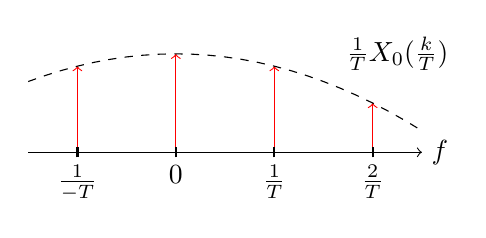
\begin{tikzpicture}[scale=1.25,
        dot/.style={circle,fill=black,minimum size=3pt,inner sep=0pt,
            outer sep=-1pt}]
	\draw[->] (-1.5,0) -- (2.5,0) node[right] {$f$};
    	
\draw[->, color=red] (-1,0) -- (-1,0.875);
\draw[->, color=red] (0,0) -- (0,1);
\draw[->, color=red] (1,0) -- (1,0.875);
\draw[->, color=red] (2,0) -- (2,0.5);

\draw[color=black, dashed, domain=-1.5:2.5]   plot (\x,{-(1/8*\x*\x)+1});
\node (note1) at (2.25,1.0)   {$\frac{1}{T}X_0(\frac{k}{T})$}; 

    
\draw[thick] (-1,-1.5pt) -- (-1,1.5pt) node[below=1mm] {$\frac{1}{-T}$};
\draw[thick] (0,-1.5pt) -- (0,1.5pt) node[below=1mm] {$0$};
\draw[thick] (1,-1.5pt) -- (1,1.5pt) node[below=1mm] {$\frac{1}{T}$};
\draw[thick] (2,-1.5pt) -- (2,1.5pt) node[below=1mm] {$\frac{2}{T}$};	
\end{tikzpicture}}
\end{tabular}

\begin{tabular}{ll}
 \addtolength{\jot}{2mm}
 \parbox{7cm}{
 \textbf{Beispiel:}\\
\begin{eqnarray*}
\text{Grundfunktion:} \quad x_0(t) &=& \alpha \cdot rect(\frac{t}{\frac{T}{4}})\\
\text{periodische Funktion:} \quad x(t) &=& \alpha \cdot rect(\frac{t}{\frac{T}{4}}) \ast  \text{\SHT}_T(t)
\end{eqnarray*}}
 &
 \parbox{5cm}{
 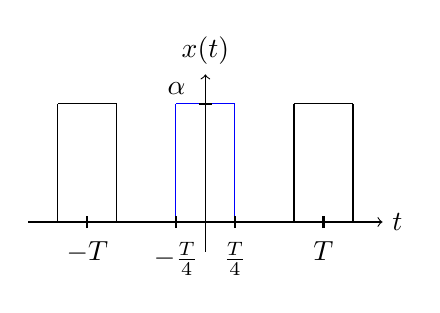
\begin{tikzpicture}[scale=1.5,
        dot/.style={circle,fill=blue,minimum size=3pt,inner sep=0pt,
            outer sep=-1pt},domain=0:4]
\draw[->] (-1.5,0) -- (1.5,0) node[right] {$t$};
\draw[->] (0,-0.25) -- (0,1.25) node[above] {$x(t)$};

\draw[color=blue] (-0.25,0) -- (-0.25,1);
\draw[color=blue] (-0.25,1) -- (0.25,1);
\draw[color=blue] (0.25,0) -- (0.25,1);

\draw[color=black] (-1.25,0) -- (-1.25,1);
\draw[color=black] (-1.25,1) -- (-0.75,1);
\draw[color=black] (-0.75,0) -- (-0.75,1);

\draw[color=black] (0.75,0) -- (0.75,1);
\draw[color=black] (0.75,1) -- (1.25,1);
\draw[color=black] (1.25,0) -- (1.25,1);

\draw[thick] (-0.25,-1.5pt) -- (-0.25,1.5pt) node[below=2mm] {$- \frac{T}{4}$};
\draw[thick] (0.25,-1.5pt) -- (0.25,1.5pt) node[below=2mm] {$\frac{T}{4}$};
\draw[thick] (-1,-1.5pt) -- (-1,1.5pt) node[below=2mm] {$-T$};
\draw[thick] (1,-1.5pt) -- (1,1.5pt) node[below=2mm] {$T$};

\draw[thick] (-1.5pt,1) -- (1.5pt,1) node[above=2mm, left=2mm] {$\alpha$};         
\end{tikzpicture}}
\end{tabular}
Durch Umformung  im Zeitbereich kann der Fouriekoeffizient ermittelt werden:
\begin{tabular}{ll}
 \addtolength{\jot}{2mm}
 \parbox{7cm}{
\begin{eqnarray*}
x(t) ~  \laplace ~ X(f) &=& \frac{ T}{4} \cdot 2 \alpha \cdot si(\frac{T}{4} \cdot 2 \pi f) \cdot \frac{1}{T} \text{\SHT}_{\frac{1}{T}}(f)\\
&=& \frac{\alpha}{2} \cdot si(\frac{T}{2} \pi f) \cdot \text{\SHT}_{\frac{1}{T}}(f)\\
&=& \frac{\alpha}{2} \cdot si(\frac{T}{2} \pi f) \cdot  \delta(f-\frac{k}{T})\\
&=& \sum_{k~\in~\mathbb{Z}} \frac{\alpha}{2} \cdot si(\frac{T}{2} \pi \frac{k}{T}) \cdot  \delta(f-\frac{k}{T})\\
&=& \sum_k \frac{\alpha}{2} \cdot si(\frac{\pi}{2}k) \cdot  \delta(f-\frac{k}{T})\\
&\Rightarrow& c_k = \frac{\alpha}{2} \cdot si(\frac{\pi}{2}k)
\end{eqnarray*}}
 &
 \parbox{5cm}{
 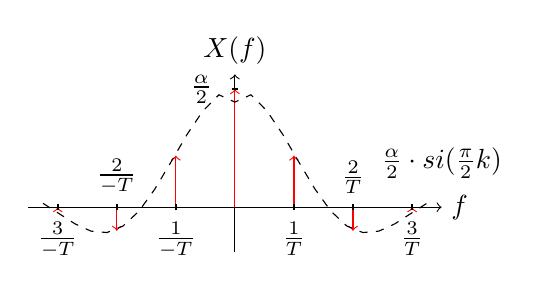
\begin{tikzpicture}[scale=0.75,
        dot/.style={circle,fill=black,minimum size=3pt,inner sep=0pt,
            outer sep=-1pt}]
	\draw[->] (-3.5,0) -- (3.5,0) node[right] {$f$};
 \draw[->] (0,-0.75) -- (0,2.25) node[above] {$X(f)$};
    	
\draw[->, color=red] (-3,0) -- (-3,0);
\draw[->, color=red] (-2,0) -- (-2,-0.4);
\draw[->, color=red] (-1,0) -- (-1,0.875);
\draw[->, color=red] (0,0) -- (0,2);
\draw[->, color=red] (1,0) -- (1,0.875);
\draw[->, color=red] (2,0) -- (2,-0.4);
\draw[->, color=red] (3,0) -- (3,0);

\draw[color=black, dashed, domain=-3.25:3.25]   plot (\x,{2*(sin(2*\x r))/(2*\x)});
\node (note1) at (3.5,0.75)  {$\frac{\alpha}{2} \cdot si(\frac{\pi}{2}k)$}; 

\draw[thick] (-3,-1.5pt) -- (-3,1.5pt) node[below=1mm] {$\frac{3}{-T}$};  
\draw[thick] (-2,-1.5pt) -- (-2,1.5pt) node[above] {$\frac{2}{-T}$};    
\draw[thick] (-1,-1.5pt) -- (-1,1.5pt) node[below=1mm] {$\frac{1}{-T}$};
\draw[thick] (1,-1.5pt) -- (1,1.5pt) node[below=1mm] {$\frac{1}{T}$};
\draw[thick] (2,-1.5pt) -- (2,1.5pt) node[above] {$\frac{2}{T}$};
\draw[thick] (3,-1.5pt) -- (3,1.5pt) node[below=1mm] {$\frac{3}{T}$};

\draw[thick] (-1.5pt,2) -- (1.5pt,2) node[left=2mm] {$\frac{\alpha}{2}$};  

\end{tikzpicture} 
 }
\end{tabular}\\~
\vfill\columnbreak
\subsection{Rechnenregeln für Fourietransformationen}
Allgemein gilt für die Transformation folgender Satz:
\begin{eqnarray*}
y(t) = \sum^{\infty}_{n = - \infty} c_n e^{j2 \pi n f_0 t} &\Rightarrow& c_n = \frac{1}{T_0} \int^{T_0}_0 y(t) e^{-j2 \pi n f_0 t}dt\\
y(t) = \int^{\infty}_{- \infty} Y(f) e^{j2 \pi n f_0 t}df  &\Rightarrow& Y(f) = \int^{\infty}_{- \infty} y(t) e^{-j2 \pi n f_0 t}dt 
\end{eqnarray*}
Desweiteren gelten noch folgende Rechenregeln und Definitionen:
\begin{tabular}{ll}
 \addtolength{\jot}{2mm}
 \parbox{6cm}{\begin{eqnarray*}
 \delta(t) &\laplace& 1\\
 rect(t) &\laplace& 2\cdot si(2 \pi f)\\
\triangle(t) &\laplace& si^2(\pi f)\\
\text{Signum:} \quad sgn(t) &\laplace& \frac{1}{j \pi f}\\
\text{\SHT}_t(t) &\laplace& \frac{1}{\vert T \vert} \text{\SHT}_{\frac{1}{T}}(f)\\
\xi(t) \cdot e^{-\alpha t} &\laplace& \frac{1}{\alpha + k2 \pi f}\\
e^{-\pi t^2}  &\laplace& e^{-\pi f^2}\\
e^{-(-t)} \xi(-t) = \xi(-t) e^t &\laplace& \frac{1}{1-j2 \pi f}\\
\int_{-\infty}^t s(\tau)d\tau &\laplace& \left(\frac{1}{2}\delta(f) + \frac{1}{j2 \pi f} \right) S(f)\\
\text{C: } \frac{1}{C} \int_{-\infty}^t i(\tau) d\tau &\laplace& \frac{1}{j2 \pi f C} I(f) \quad I(0) = 0\\
s_1(t) \ast s_2(t) &\laplace& S_1(f) \cdot S_2(f)\\
s_1(t) \cdot s_2(t) &\laplace& S_1(f) \ast S_2(f)\\
s(jt) &\laplace& 2 \pi S(-f) \\
s(-t) &\laplace& S(-f) = S^\ast(f)\\
s^\ast(t) &\laplace& S^\ast(-f)
 \end{eqnarray*}
}
 &
 \addtolength{\jot}{2mm}
 \parbox{5cm}{\begin{eqnarray*}
2 si(2 \pi t) &\laplace&  rect(-f) = rect(f)\\
cos(2 \pi f_0 t) &\laplace& \frac{1}{2}\left[ \delta(f-f_0) + \delta(f+f_0)\right] \\
\frac{1}{2} cos(4 \pi f_0 t) &\laplace& \frac{1}{8}\left[ \delta(f-2f_0) + \delta(f+2f_0)\right] \\
sin(2 \pi f_0 t) &\laplace& \frac{1}{2j}\left[ \delta(f-f_0) - \delta(f+f_0)\right] \\
\alpha_1 s_1(t) + \alpha_2 s_2(t) &\laplace& \alpha_1 S_1(f) + \alpha_2 S_2(f)\\
s(t-t_0) &\laplace& S(f) e^{-j2 \pi t_0 f}\\
s(t) e^{-j2 \pi f_0 t} &\laplace& S(f-f_0)\\
s(\alpha t) &\laplace& \frac{1}{\vert \alpha \vert} S\left( \frac{f}{\alpha}\right)\\
\frac{d}{dt}s(t) &\laplace& j2 \pi f \cdot S(f)\\
-j2 \pi f \cdot s(t) &\laplace&  \frac{d}{df} S(f)\\
\int^t_{-\infty} s(t) dt &\laplace& \frac{S(f)}{j2 \pi f} + \frac{S(0)}{2}\delta(f)\\
\frac{1}{\vert \tau \vert} si\left( \pi \cdot \frac{t}{\tau} \right) &\laplace&  rect(\tau f)
 \end{eqnarray*}}
\end{tabular}\\~
\begin{tabular}{ll}
 \addtolength{\jot}{2mm}
 \parbox{7cm}{
 Die \textbf{Dualität} oder Abbildbarkeit beschreibt das Verhalten zwischen Zeit- und Frequenzbereich und umgedreht. 
\begin{equation*}
x(t) ~\laplace~ Y(f) \Leftrightarrow y(t)~ \laplace~ X(-f)
\end{equation*}
}&
 \parbox{5cm}{
\textbf{Parsevaltheorem} beschreibt den Zusammenhang zwischen Signalenergien im Zeitbereich und im Frequenzbereich
 \begin{equation*}
\int^\infty_{-\infty} x(t) \cdot y^*(t) dt = \int^\infty_{-\infty} X(f) \cdot Y^*(f) df 
\end{equation*}
}
\end{tabular}\\
\textbf{Beispiel:} \quad Zeitverschiebung und Linearität 
\begin{eqnarray*} 
rect(2t) - \triangle(t) &\laplace& \frac{1}{2} ~2 ~si(\frac{1}{2}~2 \pi f) - si^2(\pi f) = si(\pi f) - si^2(\pi f)
\end{eqnarray*}
\subsection{Eigenschaften der Fourietransformation}
\begin{tabular}{ll}
 \addtolength{\jot}{2mm}
 \parbox{8cm}{
  \centering
\textbf{Grenzwerte von S(f)}(Lemma von Riemann-Lebesgue)
\flushleft
Da die Fourier-Transformationen von integrablen Funktionen stetig sind, handelt es sich bei der Fourietransformierten um eine stetige Funktion, die im Unendlichen verschwindet. Schnelles integrieren über positive und negative Teile der Fourietransformierten.
}
 &
 \parbox{4cm}{
 \begin{eqnarray*}
S(\infty) = S(- \infty) &=& 0\\
s(\infty) = s(- \infty) &=& 0
 \end{eqnarray*}
}
\end{tabular}\\
\vspace{6pt}
\begin{tabular}{ll}
 \addtolength{\jot}{2mm}
 \parbox{7cm}{
  \centering
\textbf{Linearität}
\flushleft
Die Fouriertransformation stellt einen linearen Operator da
}
 &
 \parbox{5cm}{
 \begin{eqnarray*}
\alpha_1 s_1(t) + \alpha_2 s_2(t)  &\laplace& \alpha_1 S_1(f) + \alpha_2 S_2(f)
 \end{eqnarray*}
}
\end{tabular}\\
\vspace{6pt}
\begin{tabular}{ll}
 \addtolength{\jot}{2mm}
 \parbox{7cm}{
  \centering
\textbf{konjungiert komplexe Zeitfunktion}
 \begin{eqnarray*}
S(f) &\laplace& \int_\mathbb{R}s(t)~e^{j2 \pi ft}dt\\
S_1(f) &=& \int_\mathbb{R}s_1(t)~e^{j2 \pi ft}dt = \int_\mathbb{R}s^*(t)~e^{j2 \pi ft}dt\\
&=& \left( \int_\mathbb{R}s(t)~e^{-j2 \pi ft}dt\right)^* = \left[ S(-f)\right]^*\\
&=& S^*(-f)
 \end{eqnarray*}
}
 &
 \parbox{5cm}{
 \begin{eqnarray*}
\text{Falls:}~ s(t) \in \mathbb{R} \forall t &\Leftrightarrow& Im\lbrace s(t)\rbrace =0\\
\Rightarrow s(t) &=& s^*(t)\\
\Rightarrow S(f) &=& S^*(-f)  \\
\vert S(f) \vert &=& \vert S(-f) \vert \quad(gerade Fkt.)\\
 s^*(t) &\laplace& S^*(-f)
 \end{eqnarray*}
}
\end{tabular}\\
\vspace{6pt}
\begin{tabular}{ll}
 \addtolength{\jot}{2mm}
 \parbox{7cm}{
  \centering
\textbf{konjungiert komplexe Frequenzfunktion}
\flushleft
siehe hierzu Rechenregeln.
}
 &
 \parbox{5cm}{
 \begin{eqnarray*}
s^*(-t) &\laplace& S*(f)
 \end{eqnarray*}
}
\end{tabular}\\
\vspace{6pt}
\begin{tabular}{ll}
 \addtolength{\jot}{2mm}
 \parbox{7cm}{
   \centering
\textbf{Reellwertige und imaginäre Funktionen}
\flushleft
\begin{align*}
x(t)  ~&\text{ungerade} &\Rightarrow& ~&X(f) ~\text{imaginär}\\
x(t)  ~&\text{gerade} &\Rightarrow& ~&X(f) ~\text{reellwertig}
\end{align*}
Der Beweis, ob eine Funktion die reelwertig oder imaginär ist, kann mittels der konjugiert komplexen der Zeitfunktion oder der Frequenzfunktion ermittelt werden.
}
 &
 \parbox{5cm}{
 Beweis, das eine reellwertige Funktion $x(t)$ eine grade Funktion ist.
 \begin{eqnarray*}
x(t) &=& \int e^{j2 \pi ft} \cdot X(f) df\\
 &=& \left[ \int \left( e^{j2 \pi ft} \cdot  X(f)\right)^*  df \right]^* \\
  &=& \left[ \int e^{-j2 \pi ft} \cdot \underbrace{X^*(f)}_\text{$=X(f)$, da reellwertig} df \right]^* \\
  \left[x(-t) \right]^* &=& x(-t)\text{, da $x(t)$ reellwertig}
 \end{eqnarray*}
}
\end{tabular}\\

\vspace{6pt}
\begin{tabular}{ll}
 \addtolength{\jot}{2mm}
 \parbox{7cm}{
  \centering
\textbf{Reellwertige Funktonen}
\flushleft
Graphisch ist $S^*(-f)$ die Spiegelung an der y-Achse, da es keine negativen Frequenzen gibt. (Bei komplexen Fkt. nicht!).
}
 &
 \parbox{5cm}{
 \begin{eqnarray*}
s(t) \in \mathbb{R} \Rightarrow s(t) &=& s^*(t) ~ \forall t \in \mathbb{R}\\
S(-f) &=& S^*(f)
 \end{eqnarray*}
}
\end{tabular}\\
\vspace{6pt}
\begin{tabular}{ll}
 \addtolength{\jot}{2mm}
 \parbox{7cm}{
  \centering
\textbf{Imaginäre Funktonen}
\flushleft
Analog zum vorherigen. Bei imaginären Funktionen ist gibt es keine Spiegelung!
}
 &
 \parbox{5cm}{
 \begin{eqnarray*}
s(t) \in \mathbb{R} \Rightarrow s(t) &=& -s^*(t) ~ \forall t \in \mathbb{R}\\
S(-f) &=& -S^*(f)
 \end{eqnarray*}
}
\end{tabular}\\~
\vfill\columnbreak
\begin{tabular}{ll}
 \addtolength{\jot}{2mm}
 \parbox{6cm}{
  \centering
\textbf{Spiegelung am Ursprung}
\begin{eqnarray*}
s(t) &\laplace& S(-f)
\end{eqnarray*}
Beweis siehe Seite.
}
 &
 \parbox{5cm}{
 \begin{eqnarray*}
 F \lbrace s(-t)\rbrace &=& \int_\mathbb{R} s(-t) e^{-j2 \pi ft} dt \qquad \text{mit $-t = \tau$}\\
F \lbrace s(\tau)\rbrace&=& \int_{-\infty}^\infty s(\tau) e^{-j2 \pi f \tau} (-d\tau)\\
&=& \int_\mathbb{R} s(-t) e^{j2 \pi ft} dt = S(-f)
 \end{eqnarray*}
}
\end{tabular}\\
\vspace{6pt}
\begin{tabular}{ll}
 \addtolength{\jot}{2mm}
 \parbox{5cm}{
  \centering
\textbf{Zeitverschiebung}
\begin{eqnarray*}
s(t-t_0) &\laplace& S(f) \cdot e^{-j2 \pi f t_0}
\end{eqnarray*}
Folgt durch Substitution mit zeitlicher Verschiebung um $t_0$ \\(Phaseninformation ändert sich).
}
 &
 \parbox{5cm}{
 \begin{eqnarray*}
 F \lbrace s(t-t_0)\rbrace &=& \int_\mathbb{R} s(t-t_0) ~e^{-j2 \pi ft} dt \qquad \text{mit $\tau = t-t_0$}\\
&=& \int_\mathbb{R} s(\tau) ~e^{-j2 \pi f (\tau + t_0)} d\tau \qquad \text{mit $t = \tau$}\\
&=&  e^{-j2 \pi f t_0} \cdot \int_\mathbb{R} s(t) ~e^{-j2 \pi ft} dt
 \end{eqnarray*}
}
\end{tabular}\\
\begin{tabular}{ll}
 \addtolength{\jot}{2mm}
 \parbox{5cm}{
  \centering
\textbf{Frequenzverschiebung}
\begin{eqnarray*}
s(t) \cdot e^{j2 \pi f t_0} &\laplace& S(f-f_0)
\end{eqnarray*}
Verschiebung von z.B. Radiosignalen in den hörbaren Bereich
}
 &
 \parbox{5cm}{

\begin{eqnarray*}
s(t) \cdot cos(2 \pi f_0t) &\laplace& \frac{1}{2}\left[ S(f+f_0) + S(f-f_0)\right] 
\end{eqnarray*}
Bsp: Modulation einer sinusförmigen Welle gemäß der Gleichung. Jede Verschiebung von $f_0$ hat eine Verschiebung von $-f_0$ zur folge.
}
\end{tabular}\\
\vspace{6pt}
\begin{tabular}{ll}
 \addtolength{\jot}{2mm}
 \parbox{4cm}{
  \centering
\textbf{Zeitskalierung}
\begin{eqnarray*}
s(\alpha t) \cdot \frac{1}{\alpha} S\left( \frac{f}{\alpha}\right) \qquad \alpha \ne 0 
\end{eqnarray*}
\flushleft
Wenn $\alpha > 1$~ wird die Zeit komprimiert, wenn $\alpha < 1$ wird die Zeit gedehnt. Bei $\alpha = 2$ wird so die Frequenz verdoppelt, das Spektrum wird im zwei auseinander gezogen.
}
 &
 \parbox{5cm}{
\begin{eqnarray*}
F\lbrace \underbrace{s(\alpha t)}_{=\tilde{s}(t)} \rbrace &\laplace& \tilde{S}(f)\\
&=& \int_\mathbb{R} s(\alpha t) ~e^{-j2 \pi ft} dt \qquad \text{mit $t = \frac{\tau}{\alpha}$}\\
&=& \begin{cases} 
a > 0: ~  \displaystyle \int_{-\infty}^{\infty} s(\tau) e^{-j2 \pi f \frac{\tau}{\alpha}}~ \frac{d\tau}{\alpha} = \frac{1}{\alpha} S\left( \frac{f}{\alpha}\right) \\[2em]
a < 0: ~  \displaystyle \int_{\infty}^{-\infty} s(\tau) e^{-j2 \pi f \frac{\tau}{\alpha}}~ \frac{d\tau}{\alpha} = \frac{1}{- \alpha} S\left( \frac{f}{\alpha}\right) \\[2em]
\end{cases}\\
&\Rightarrow& \frac{1}{\vert \alpha \vert} S\left( \frac{f}{\alpha} \right) 
\end{eqnarray*}
}
\end{tabular}\\~
\vspace{6pt}
\flushleft
\textbf{1. Beispiel:} \quad Darstellung der Dreiecksfunktion im Zeitbereich durch Faltung zweier Rechtecke
\begin{eqnarray*} 
s(t) = \triangle \left( \frac{t}{T} \right) &=& \frac{1}{T} \cdot rect \left(\frac{2t}{T} \right) \ast rect \left(\frac{2t}{T} \right) 
\end{eqnarray*}\\
\textbf{2. Beispiel:} \quad Dualitätsbeziehungen zwischen Frequenz- und Zeitbereich
\begin{eqnarray*} 
si\left( \frac{t}{2}\right) = si\left( \frac{2  \pi t}{4 \pi }\right) &\laplace&  \frac{4 \pi}{2} \cdot rect\left( \frac{- 4 \pi f}{2}\right)  = 2 \pi \cdot rect(2 \pi f) \qquad \Rightarrow \text{idealer Tiefpass}
\end{eqnarray*}\\~
\subsection{Abtasttheorem \& Rekonstruktion}
\begin{tabular}{ll}
 \addtolength{\jot}{2mm}
 \parbox{6cm}{
 Durch dieses Theorem beschreibt die eindeutige Wandlung von zeitkontinuierliche Signale in zeitdiskrete Signale.
\begin{equation*}
s(t) \quad t ~\in~\mathbb{R} \Rightarrow s(nT) \quad n ~\in~\mathbb{Z}
\end{equation*} 
Die Abtastrate zwischen den Abtastwerten beträgt $\frac{1}{T}$. Bei beliebigen Signalen ist man nicht in der Lage diese eindeutig zu bestimmen.
}
 &
 \parbox{5cm}{
 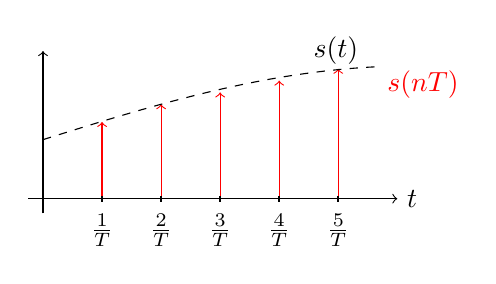
\begin{tikzpicture}[scale=0.75,
        dot/.style={circle,fill=black,minimum size=3pt,inner sep=0pt,
            outer sep=-1pt}]
\draw[->] (-0.25,0) -- (6,0) node[right] {$t$};
 \draw[->] (0,-0.25) -- (0,2.5) node[above] {};
    	
\draw[->, color=red] (1,0) -- (1,1.3);
\draw[->, color=red] (2,0) -- (2,1.6);
\draw[->, color=red] (3,0) -- (3,1.8);
\draw[->, color=red] (4,0) -- (4,2);
\draw[->, color=red] (5,0) -- (5,2.2) node[below=2mm, right=5mm] {$s(nT)$};

\draw[color=black, dashed, domain=0:5.75]   plot (\x,{1.25*(sin(0.25*\x r))+1})node[above=2mm, right=-10mm]{$s(t)$}; 

\draw[thick] (1,-1.5pt) -- (1,1.5pt) node[below=1mm] {$\frac{1}{T}$};
\draw[thick] (2,-1.5pt) -- (2,1.5pt) node[below=1mm] {$\frac{2}{T}$};
\draw[thick] (3,-1.5pt) -- (3,1.5pt) node[below=1mm] {$\frac{3}{T}$};
\draw[thick] (4,-1.5pt) -- (4,1.5pt) node[below=1mm] {$\frac{4}{T}$};
\draw[thick] (5,-1.5pt) -- (5,1.5pt) node[below=1mm] {$\frac{5}{T}$}; 

\end{tikzpicture} 
}
\end{tabular}\\
\begin{eqnarray*}
u(t) = \sum_{k \in \mathbb{Z}} ~s(kT) \cdot \delta(t-kT) = s(T) \cdot \text{\SHT}_T (t) &\laplace& U(f) = S(f) \cdot\frac{1}{T} \text{\SHT}_\frac{1}{T} (f)
\end{eqnarray*}
In der spektralen Darstellung wird ersichtlich, das die Funktion aus mehreren kopierten $S(f)$ besteht.
\begin{tabular}{ll}
 \addtolength{\jot}{2mm}
 \parbox{6cm}{
 \begin{tikzpicture}[scale=0.75,
        dot/.style={circle,fill=black,minimum size=3pt,inner sep=0pt,
            outer sep=-1pt}]
\draw[->] (-2.5,0) -- (2.5,0) node[right] {$f$};
\draw[->] (0,-0.25) -- (0,2.5) node[above] {$S(f)$};
   
\draw[color=blue] (-2,0) -- (-2,2);
\draw[color=blue] (-2,2) -- (2,2);
\draw[color=blue] (2,0) -- (2,2);
 	
\draw[thick] (-2,-1.5pt) -- (-2,1.5pt) node[below=1mm] {$-W$};
\draw[thick] (2,-1.5pt) -- (2,1.5pt) node[below=1mm] {$W$};

\end{tikzpicture} 
}
 &
 \parbox{5cm}{
 \begin{tikzpicture}[scale=0.75,
        dot/.style={circle,fill=black,minimum size=3pt,inner sep=0pt,
            outer sep=-1pt}]
	\draw[->] (-3.5,0) -- (3.5,0) node[right] {$f$};
 \draw[->] (0,-0.25) -- (0,2.5) node[above] {$U(f)$};
    	
\draw[color=black] (-2.5,0) -- (-2.5,2);
\draw[color=black] (-2.5,2) -- (-1.5,2);
\draw[color=black] (-1.5,0) -- (-1.5,2);

\draw[color=blue] (-0.5,0) -- (-0.5,2);
\draw[color=blue] (-0.5,2) -- (0.5,2);
\draw[color=blue] (0.5,0) -- (0.5,2);

\draw[color=black] (1.5,0) -- (1.5,2);
\draw[color=black] (1.5,2) -- (2.5,2);
\draw[color=black] (2.5,0) -- (2.5,2);

\draw[thick] (-2,-1.5pt) -- (-2,1.5pt) node[below=1mm] {$\frac{-1}{T}$};
\draw[thick] (2,-1.5pt) -- (2,1.5pt) node[below=1mm] {$\frac{1}{T}$};
\draw[thick] (-1.5pt,2) -- (1.5pt,2) node[right=5mm] {$\frac{1}{T}$};

\end{tikzpicture} 
}
\end{tabular}\\
\begin{tabular}{ll}
 \addtolength{\jot}{2mm}
 \parbox{6cm}{
Es ist darauf zu achten, das die doppelte Bandbreite $W$ des transformierten Signals $U(f)$ kleiner ist, als die Abtastfrequenz $\frac{1}{T}$, da sonst Aliasing Effekte entstehen können. Diese sind im Frequenzbereich durch Überlappungen sichtbar (siehe schraffierte Bereiche)
}
 &
 \parbox{5cm}{
 \begin{tikzpicture}[scale=0.75,
        dot/.style={circle,fill=black,minimum size=3pt,inner sep=0pt,
            outer sep=-1pt}]
	\draw[->] (-4,0) -- (4,0) node[right] {$f$};
 \draw[->] (0,-0.25) -- (0,3) node[above] {$U(f)$};
    	
\draw[color=black, dashed] (-2,2.5) -- (-4,2.5);    	
\draw[color=black] (-2,2.5) -- (-0.5,2.5);
\draw[color=black] (-0.5,0) -- (-0.5,2.5);

\draw[color=black] (0.5,0) -- (0.5,2.5);
\draw[color=black] (0.5,2.5) -- (2,2.5);
\draw[color=black, dashed] (2,2.5) -- (4,2.5);

\draw[color=red, thick] (-1.5,0) -- (-1.5,2.5);
\draw[color=red, thick] (-1.5,2.5) -- (1.5,2.5);
\draw[color=red, thick] (1.5,0) -- (1.5,2.5);

\draw[thick] (-1.5,-1.5pt) -- (-1.5,1.5pt) node[below=1mm] {$-W$};
\draw[thick] (1.5,-1.5pt) -- (1.5,1.5pt) node[below=1mm] {$W$};
\draw[thick] (-2.5,-1.5pt) -- (-2.5,1.5pt) node[above=1mm] {$\frac{-1}{T}$};
\draw[thick] (2.5,-1.5pt) -- (2.5,1.5pt) node[above=1mm] {$\frac{1}{T}$};

\draw[pattern=north west lines, pattern color=blue] (1.5,0) rectangle (0.5,2.5);
\draw[pattern=north east lines, pattern color=blue] (-1.5,0) rectangle (-0.5,2.5);

\end{tikzpicture} 
}
\end{tabular}
\begin{tabular}{ll}
 \addtolength{\jot}{2mm}
 \parbox{6cm}{
Es muss $\frac{1}{T} $>$ 2W$ gelten, damit $s(t)$ eindeutig reproduzierbar ist. Zudem müssen die kopierten Signale von $S(f)$ durch die \SHT-Funktion (z.B. $S(f-\frac{1}{T})$,~$S(f-\frac{2}{T})$,~...) ausgeblendet werden durch einen idealen Tiefpass (si-Funktion im Zeitbereich).
}
 &
 \parbox{5cm}{
 \centering
 \textbf{Nyquist-Theorem:}
 \begin{eqnarray*} 
s(t) &=& \sum s(nT) \cdot \underbrace{si\left( \pi \cdot \frac{t-nT}{T} \right)}_\text{idealer Tiefpass}
\end{eqnarray*}
}
\end{tabular}
\vspace{6pt}\\~
\textbf{1. Beispiel:} \quad Abtastung von $s(t)$ und Rekonstruktion $\tilde{s}(t)$  mit einem Rekonstruktionsfilter $c_1(t)$
\begin{eqnarray*} 
\tilde{s}(t) &=& \left(s(t) \cdot \text{\SHT}_T (t) \right) \ast c_1(t) ~ = \left( \sum_{k \in \mathbb{Z}} s(kT) \delta(t-kT) \right) \ast c_1(t)\\
&=& \sum_{k \in \mathbb{Z}} s(kT)\left( \delta(t-kT)  \ast c_1(t)\right) = \sum_{k \in \mathbb{Z}} s(kT)\cdot c_1(t-kT)
\end{eqnarray*}\\
\textbf{2. Beispiel:} \quad ideale Rekonstruktion $\tilde{s}(t) =s(t)$  mit einem Rekonstruktionsfilter $c_2(t)$
\begin{eqnarray*} 
\tilde{S} (f) &=& S(f) \cdot \frac{1}{T} \text{\SHT}_\frac{1}{T} (f) \cdot C_2(f) = S(f) \cdot \frac{1}{T} \text{\SHT}_\frac{1}{T} (F) \cdot T~rect\left( \frac{f}{\frac{1}{2T}}\right) \\
 &\Rightarrow& T = \frac{1}{2W} \quad \text{Bestimmung von T über W darf nicht fehlen!}
\end{eqnarray*}\\
\vfill\columnbreak
\subsection{Warscheinlichkeitsrechnung}
\begin{center}
\textbf{Bedingte Wahrscheinlichkeit und Wahrscheinlichkeitsraum}
\end{center}
\begin{tabular}{ll}
 \addtolength{\jot}{2mm}
 \parbox{6cm}{
 \begin{eqnarray*}
 P(\bar{A}) &=& P(\Omega \ A) = 1- P(A)\\
 P(A) + P(B) &=& P(A \cap B) + P(A \cup B)
 \end{eqnarray*}}
 &
 \addtolength{\jot}{2mm}
 \parbox{5cm}{
 \begin{eqnarray*}
 P(A \cap B) &=& P(A)P(B \vert A) = P(B) P(A \vert B)\\
 P(B \vert A) &=& \frac{P(A \cap B)}{P(A)}
 \end{eqnarray*}}
\end{tabular}
\vspace{6pt}
\begin{center}
\textbf{Normalverteilung}
\end{center}
\begin{tabular}{ll}
 \addtolength{\jot}{2mm}
 \parbox{6cm}{
 \textbf{im $\mathbb{R}$: }
 \begin{eqnarray*}
 p(x) &=& \frac{1}{\sqrt{2 \pi \sigma^2}} e^{\frac{-(x-\mu)^2}{2 \sigma^2}}\\
\mu = E(X) &=& \int x p(x) dx \\
\sigma^2 = E((X-\mu)^2) &=& \int (x- \mu)^2 p(x) dx
 \end{eqnarray*}}
 &
 \addtolength{\jot}{2mm}
 \parbox{6cm}{
 \textbf{im $\mathbb{R}^n$ mit Kovarianzmatrix $M$: }
 \begin{eqnarray*}
 p(x_1, ... ,x_n) &=& \frac{1}{(2\pi)^{\frac{n}{2}} \sqrt{det(M)}} e^{-\frac{1}{2}(x- \mu)^T M^{-1}(x-\mu)}\\
\mu = E(X) &=& E \left[ [X_1, ... X_n]^T  \right]  \\
M &=& E \left[ (X- \mu) (X- \mu)^T \right]
\end{eqnarray*}}
\end{tabular}
Wenn $\mu = 0$ und $\sigma^2 = 1$ ist, dann spricht man von einer Standartnormalverteilung. Für diese Verteilung kann die Warscheinlichkeit mit der Q-Funktion berechnet werden.
\begin{tabular}{ll}
 \addtolength{\jot}{2mm}
 \parbox{4cm}{
 \begin{eqnarray*}
Q(x) &=& \frac{1}{\sqrt{2 \pi}} \int_{\pi}^{\infty} e^{\frac{-t^2}{2}}dt\\ 
 \end{eqnarray*}
Standartnormalverteilung: \\
$P(X \geq a) = Q(a)$ \quad $a \geq 0$ \\
Für $ a < 0$: \\
$P(X \geq a) = 1-Q(\vert a \vert)$
 }
 &
 \addtolength{\jot}{2mm}
 \parbox{5cm}{
\begin{center}
 \includegraphics[width=0.30\textwidth]{img/Q-Funktion.jpg}
\end{center}}
\end{tabular}\\
\vspace{10pt}
\textbf{1. Beispiel:} Wahrscheinlichkeiten $P(0 \leq X \leq 1), P(X \leq 2), P(-1 \leq X 2)$ mit Standartnormalverteilung
\begin{eqnarray*}
P(0 \leq X \leq 1) &=& Q(0) - Q(1) \approx 0.5 - 0.15866 \approx 0.34134\\
P(X \leq 2) &=& 1 - Q(2) \approx 1 - 0.022725 \approx 0.97725\\
P(-1 \leq X 2) &=& 1-Q(1)-Q(2) \approx 0.97725-0.15866 \approx 0.81859
\end{eqnarray*}
\vspace{10pt}
Für Normalverteilungen mit Erwartungswert $\mu$ und Varianz $\sigma^2$ gilt für $x > \mu$:
\begin{eqnarray*}
P(X \geq a) &=& \frac{1}{\sqrt{2 \pi \sigma^2}} \int_x^{\infty} e^{\frac{-(t-\mu)^2}{2 \sigma^2}} dt \overset{t' =(t-\mu)/\sigma}{=} \frac{1}{\sqrt{2 \pi \sigma^2}} \int_{(x-\mu)/ \sigma}^{\infty} e^{\frac{-t'^2}{2}} dt' = Q\left(\frac{x-\mu}{\sigma}\right) 
\end{eqnarray*}\\
\vspace{10pt}
\textbf{2. Beispiel:} Wahrscheinlichkeiten $P(0 \leq X \leq 1), P(X \leq 0))$ mit $\mu = -1, \sigma^2 = 4$
\begin{eqnarray*}
P(0 \leq X \leq 1) &=& Q\left(\frac{0- (-1)}{2}\right) -  Q\left(\frac{ 1 - (-1)}{2}\right) = Q(0.5) - Q(1) \qquad \text{Symmetrie der Glockenkurve} \\
P(X \leq 0) &=& 1 - Q\left(\frac{0 - (-1))}{2}\right)) = 1 - Q(0.5)\\
\end{eqnarray*}
\begin{center}
\textbf{Zufallsvektoren}
\end{center}
\begin{tabular}{ll}
 \addtolength{\jot}{2mm}
 \parbox{6cm}{Mehrere Zufallsvariablen können in einem Zufallsvektor gebündelt werden. Die Wahrscheinlichkeit das der Zufallsvektor in einem Gebiet $\Omega$ liegt, kann berechnet werden mit $P(\vec{X} \in \Omega)$. Im AWGN-Kanal sind die Rauschvektoren voneinander unabhängig. Wenn das Signal $\vec{r} = \vec{s}_m + \vec{n}$ empfangen wird, dann ist die Dichtefunktion $p(\vec{r} \vert \vec{s}_m)$, die Dichtefunktion von Normalverteilungen. Die letzte Formel ist für $n$ verschiedene Zufallsvariablen. 
}
 &
 \addtolength{\jot}{2mm}
 \parbox{6cm}{
 \begin{eqnarray*}
P(\vec{X} \in \Omega) &=& \int_{\Omega} p(x_1, ... x_n) dx_1 ... dx_n\\
p(\vec{r} \vert \vec{s}_m) &=& p_1(\vec{r_1} \vert \vec{s}_{m1}) \cdot ... \cdot p_n(\vec{r_n} \vert \vec{s}_{mn})\\
&=& \frac{1}{\sqrt{2 \pi \omega12}} e^{\frac{-(r_k - s_{mk})}{2 \sigma^2}}\\ 
&=& \frac{1}{(\sqrt{2 \pi \omega12})^n} e^{\frac{-(r_k - s_{mk})}{2 \sigma^2}} 
\end{eqnarray*}}
\end{tabular}
\vspace{10pt}
\textbf{3. Beispiel:} Wahrscheinlichkeiten das $\vec{s} = (\sqrt{E_g}, \sqrt{E_g})$ ein Signal welches für alle $\vec{r} \geq 0$ richtig detektiert wird. Wie groß ist die Fehlerwarscheinlichkeit für $\sigma^2 = \frac{N_0}{2}$ und $\frac{E_g}{N_0} = 2$?
\begin{eqnarray*}
p(\vec{r} \vert \vec{s}) &=& \frac{1}{2\pi \sigma^2} e^{\frac{- \Vert \vec{r} - \vec{s} \Vert^2}{2 \sigma^2}} = \frac{1}{\sqrt{2 \pi \sigma}} e^{\frac{- (\vec{r}_1 - \vec{s}_1)^2}{2 \sigma^2}} \cdot \frac{1}{\sqrt{2 \pi \sigma}} e^{\frac{- (\vec{r}_2 - \vec{s}_2)^2}{2 \sigma^2}} \\
P(\vec{r}_{\text{detektiert}} \vert \vec{s}_{\text{gesendet}}) &=& \int_0^{\infty} \int_0^{\infty}  p(\vec{r} \vert \vec{s}) dr_1 dr_2 \\
&=& \int_0^{\infty} frac{1}{\sqrt{2 \pi \sigma}} e^{\frac{- (\vec{r}_1 - \vec{s}_1)^2}{2 \sigma^2}} dr_1 \cdot \int_0^{\infty} \frac{1}{\sqrt{2 \pi \sigma}} e^{\frac{- (\vec{r}_2 - \vec{s}_2)^2}{2 \sigma^2}} dr_2 \\
&=& \left(1-Q\left(\frac{s_1}{\sigma} \right)  \right) \cdot \left(1-Q\left(\frac{s_2}{\sigma} \right)  \right)  = \left(1-Q \left(\sqrt{\frac{E_g}{N_0 /2}} \right)  \right) \cdot \left(1-Q \left(\sqrt{\frac{E_g}{N_0 /2}} \right)  \right)\\ &=& (1-Q(2))^2 \\
P(\vec{r}_{\text{falsch}} \vert \vec{s}_{\text{gesendet}}) &=& 1-(1-Q(2))^2 \approx 0.045
\end{eqnarray*}
\subsection{Analysis, Lineare Algebra Regeln}
 \begin{eqnarray*}
 \int_{\mathbb{R}} e^{\alpha \cdot t} dt &=& \frac{1}{\alpha} \cdot e^{\alpha \cdot t}\\
 \int u(x) \cdot v'(x) dx &=& u(x) \cdot v(x) - \int u'(x) \cdot v(x) dx \\
 \text{Lin. Unabhängigkeit: } 0 &=& \alpha_1 s_1(t) + \alpha_2 s_2(t) \qquad \text{unab. nur bei $\alpha_1 = \alpha_2 = 0$}
  \end{eqnarray*}

\vfill

\columnbreak

\section{Modulationen} 
\subsection{Amplitudenmodulation}
\begin{tabular}{ll}
 \addtolength{\jot}{2mm}
 \parbox{6cm}{
 Bei der Amplitudenmodulation wird die Amplitude eines Träger mit der Frequenz $f_0$ um das Informationssignal $s(t)$ variiert.
 \begin{eqnarray*}
 x(t) &=& A(t) \cdot cos(2 \pi f_0t)\\
 &=& A\left[1+m\cdot s_1(t)\right]cos(2 \pi f_0t)
 \end{eqnarray*}
 Der Koeffizient m dient zur Normierung, sodass gilt, das die Amplitude niemals negativ wird und maximal den Wert 2 annehmen kann.
 \begin{eqnarray*}
 0 < m < 1 &\Rightarrow& max \vert s_1(t) \vert = 1
 \end{eqnarray*}
 Die Normierung muss stattfinden, damit es keine negative Amplitude und somit keinen Phasensprung gibt.
 \vspace{6pt}
 \\Im Frequenzbereich wird die fouriertransformierte des Signals $s(t)$ um die Diracs der Kosinusfunktion gefaltet bzw. verschoben. Wichtig ist hierbei das die Höhe des Signals halbiert wird. Die fourietransformierte des Signals kann durch zwei Seitenbänder dargestellt werden, diese sind auf der komplexen Ebene sehr gut zu sehen.
  \begin{eqnarray*}
 x(t) &\laplace& A(f) \ast \frac{1}{2} \left[\delta(f-f_0) + \delta(f+f_0) \right]\\
  x(t) &\laplace& S(f) \ast \frac{Am}{2} \left[\delta(f-f_0) + \delta(f+f_0) \right]\\
   x(t) &\laplace& \underbrace{\frac{A}{2} \delta(f-f_0) + \frac{Am}{2} s(f-f_0)}_{\text{unteres Seitenband}} + \underbrace{\frac{A}{2} \delta(f+f_0) + \frac{Am}{2} s(f+f_0)}_{\text{oberes Seitenband}}
 \end{eqnarray*} 
}
 &
 \parbox{5cm}{
 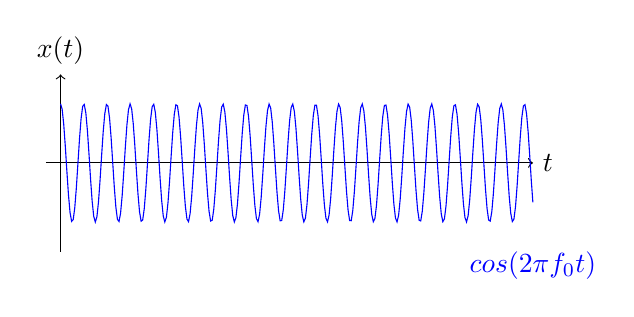
\begin{tikzpicture}[scale=0.75,
        dot/.style={circle,fill=black,minimum size=3pt,inner sep=0pt,
            outer sep=-1pt}]
	\draw[->] (-0.25,0) -- (8,0) node[right] {$t$};
 \draw[->] (0,-1.5) -- (0,1.5) node[above] {$x(t)$};

\draw[color=blue, domain=0:8, samples=300]   plot(\x,{(cos(16*\x r))}) node[below=5mm]{$cos(2 \pi f_0t)$}; 

\end{tikzpicture} \\
 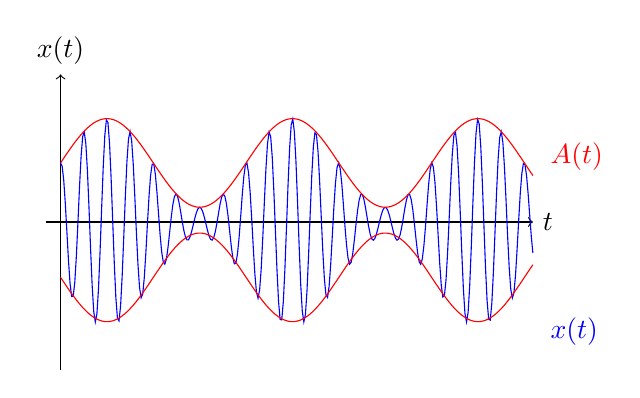
\begin{tikzpicture}[scale=0.75,
        dot/.style={circle,fill=black,minimum size=3pt,inner sep=0pt,
            outer sep=-1pt}]
	\draw[->] (-0.25,0) -- (8,0) node[right] {$t$};
 \draw[->] (0,-2.5) -- (0,2.5) node[above] {$x(t)$};

\draw[color=blue, domain=0:8, samples=300]   plot(\x,{((0.75*sin(2*\x r)+1)*(cos(16*\x r))}) node[below=10mm,  right=1mm]{$x(t)$};
\draw[color=red, domain=0:8, samples=300]   plot(\x,{((0.75*sin(2*\x r)+1)}) node[above=7, right=1mm]{$A(t)$}; 
\draw[color=red, domain=0:8, samples=300]   plot(\x,{(-0.75*(sin(2*\x r)+1.25)}); 

\end{tikzpicture} 
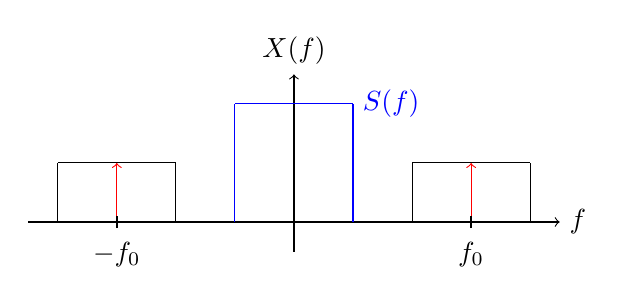
\begin{tikzpicture}[scale=1.5,
        dot/.style={circle,fill=blue,minimum size=3pt,inner sep=0pt,
            outer sep=-1pt},domain=0:4]
\draw[->] (-2.25,0) -- (2.25,0) node[right] {$f$};
\draw[->] (0,-0.25) -- (0,1.25) node[above] {$X(f)$};

\draw[color=blue] (-0.5,0) -- (-0.5,1);
\draw[color=blue] (-0.5,1) -- (0.5,1) node[right]{$S(f)$};
\draw[color=blue] (0.5,0) -- (0.5,1);


\draw[color=black] (-2,0) -- (-2,0.5);
\draw[color=black] (-2,0.5) -- (-1,0.5);
\draw[color=black] (-1,0) -- (-1,0.5);
\draw[->, color=red] (-1.5,0) -- (-1.5,0.5);

\draw[color=black] (1,0) -- (1,0.5);
\draw[color=black] (1,0.5) -- (2,0.5);
\draw[color=black] (2,0) -- (2,0.5);
\draw[->, color=red] (1.5,0) -- (1.5,0.5);

\draw[thick] (-1.5,-1.5pt) -- (-1.5,1.5pt) node[below=2mm] {$-f_0$};
\draw[thick] (1.5,-1.5pt) -- (1.5,1.5pt) node[below=2mm] {$f_0$};        
\end{tikzpicture}\\
\vspace{40pt}}
\end{tabular}\\~
\begin{tabular}{ll}
 \parbox{6cm}{
 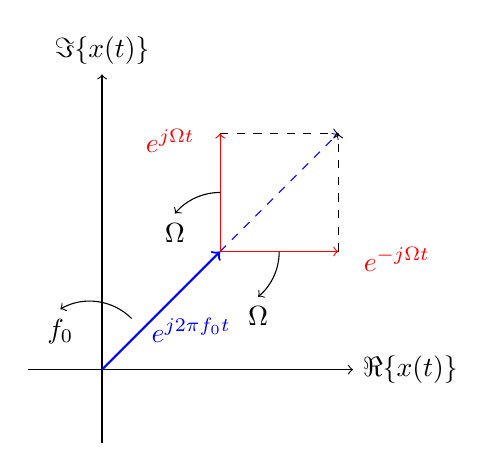
\begin{tikzpicture}[scale=0.75,
        dot/.style={circle,fill=blue,minimum size=3pt,inner sep=0pt,
            outer sep=-1pt},domain=0:4]
\draw[->] (-1.25,0) -- (4.25,0) node[right] {$\Re\lbrace x(t)\rbrace$};
\draw[->] (0,-1.25) -- (0,5) node[above] {$\Im\lbrace x(t)\rbrace$};

\draw[->, color=blue,thick] (0,0) -- (2,2) node[below=10mm, right=-10mm]{$e^{j2 \pi f_0 t}$};
\draw[->]  (60:1) arc (45:120:1) node[below] {$f_0$}; 
\draw[->, dashed,color=blue] (2,2) -- (4,4);      

\draw[->, dashed] (2,4) -- (4,4); 
\draw[->, color=red] (2,2) -- (2,4) node[below=1mm, left=2mm]{$e^{j \Omega t}$};
\draw[->]  (2,3) arc (90:140:1) node[below] {$\Omega$};       

\draw[->, dashed] (4,2) -- (4,4); 
\draw[->, color=red] (2,2) -- (4,2) node[below=1mm, right=2mm]{$e^{-j \Omega t}$};
\draw[->]  (3,2) arc (0:-50:1) node[below] {$\Omega$};

\end{tikzpicture}\\~
}&
 \parbox{7cm}{
 Im komplexen besteht die Modulation aus zwei Seitenbändern die sich gegeneinander mit der  Frequenz $\Omega$ drehen.
 \begin{eqnarray*} 
s(t) &=& cos(\Omega t) = \frac{1}{2} \left[ e^{j\Omega t}  + e^{-j\Omega t} \right] 
\end{eqnarray*}
Zudem ist es möglich zwei Signale $A(t)$ und $B(t)$ bei der gleichen Frequenz zu übertragen. Das eine Signal wird mittels $cos(\omega_0t)$ und das andere Signal mittels $sin(\omega_0t)$ moduliert. Da die beiden Träger orthogonal zueinander sind (in Quadratur) ist das die sogenannte \textbf{orthogonale Modulation}. Das Frequenzspektrum ist das gleiche, aber die einzelnen Signale mit Träger stören sich nicht gegenseitig.
 \begin{eqnarray*} 
xt) &=& A(t) \cdot cos(\omega_0t) + B(t) \cdot sin(\omega_0t)
\end{eqnarray*}
}
\end{tabular}\\~
\vspace{6pt}
\subsection{Winkelmodulation}
\begin{tabular}{ll}
 \addtolength{\jot}{2mm}
 \parbox{6cm}{
Als Winkelmodulation wird die Phasen- und Frequenzmodulation bezeichnet. Dieses Signal wird wie folgt definiert:
 \begin{eqnarray*}
 x(t) &=& A\cdot cos(2 \pi f_0t+\varphi(t))\\
 \text{PM:~}\varphi(t) &=& m \cdot s_1(t)\\
  \text{FM:~} \frac{d \varphi(t)}{dt} &=& \Delta\omega_0 \cdot s_1(t)
 \end{eqnarray*}
 Der Koeffizient $m$ dient zum bestimmen des Phasenhubs und der Koeffizient $\omega_0$ dient zur Bestimmung des Frequenzhubs. Bei der Phasenmodulation wird die Frequenz geändert. Bei der Frequenzmodulation wird das gleiche gemacht, aber technisch gesehen wird nicht die Phase sondern die Ableitung der Phase variiert. Die Fourietransformation einer Winkelmodulation hat folgende Gestalt:
  \begin{eqnarray*}
   X(f)&=&\int_\mathbb{R} A\cdot cos(2\pi f_0t + \varphi(t)) \cdot e^{-j2 \pi ft}dt\\
  X(f) &=& \frac{A}{2}\left[\psi(m,f-f_0)+ \psi(-m,f+f_0) \right] \\
\psi(m,f) &=& \int_\mathbb{R} e^{^jms_1(t)}e^{-j2 \pi ft}dt
 \end{eqnarray*} 
}
 &
 \parbox{5cm}{
 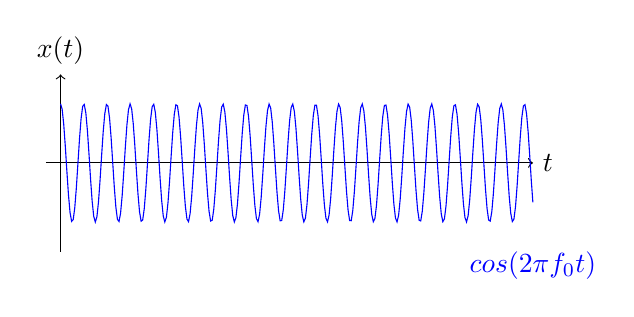
\begin{tikzpicture}[scale=0.75,
        dot/.style={circle,fill=black,minimum size=3pt,inner sep=0pt,
            outer sep=-1pt}]
	\draw[->] (-0.25,0) -- (8,0) node[right] {$t$};
 \draw[->] (0,-1.5) -- (0,1.5) node[above] {$x(t)$};

\draw[color=blue, domain=0:8, samples=300]   plot(\x,{(cos(16*\x r))}) node[below=5mm]{$cos(2 \pi f_0t)$}; 

\end{tikzpicture} \\
 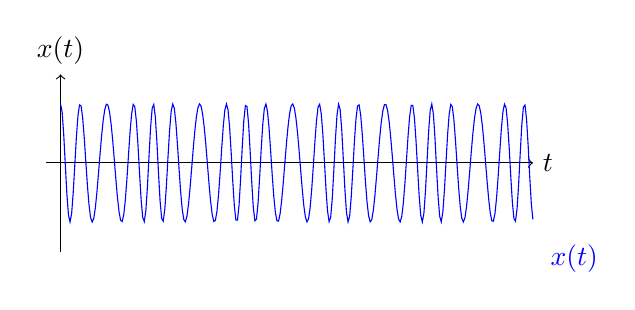
\begin{tikzpicture}[scale=0.75,
        dot/.style={circle,fill=black,minimum size=3pt,inner sep=0pt,
            outer sep=-1pt}]
	\draw[->] (-0.25,0) -- (8,0) node[right] {$t$};
 \draw[->] (0,-1.5) -- (0,1.5) node[above] {$x(t)$};

\draw[color=blue, domain=0:8, samples=300]   plot(\x,{(cos((16*\x + sin((4*\x) r)) r)}) node[below=5mm,  right=1mm]{$x(t)$};

\end{tikzpicture}
\begin{tikzpicture}[scale=1.5,
        dot/.style={circle,fill=blue,minimum size=3pt,inner sep=0pt,
            outer sep=-1pt},domain=0:4]
\draw[->] (-2.25,0) -- (2.25,0) node[right] {$f$};
\draw[->] (0,-0.25) -- (0,1.25) node[above] {$X(f)$};

\draw[color=blue] (-0.25,0) -- (-0.25,1);
\draw[color=blue] (0.25,0) -- (0.25,1) node[right]{$S(f)$};
\draw[thick] (-0.25,-1.5pt) -- (-0.25,1.5pt) node[below=2mm] {$-\Omega$};
\draw[thick] (0.25,-1.5pt) -- (0.25,1.5pt) node[below=2mm] {$\Omega$}; 
 
\draw[->, color=red] (-1.5,0) -- (-1.5,1) node[right]{$\frac{X(f)}{2}$};
\draw[color=black] (-2,0) -- (-2,0.25);
\draw[color=black] (-1.75,0) -- (-1.75,0.75);
\draw[color=black] (-1.5,0) -- (-1.5,0.5);
\draw[color=black] (-1.25,0) -- (-1.25,0.75);
\draw[color=black] (-1,0) -- (-1,0.25);

\draw[->, color=red] (1.5,0) -- (1.5,1) node[right]{$\frac{X(f)}{2}$};
\draw[color=black] (2,0) -- (2,0.25);
\draw[color=black] (1.75,0) -- (1.75,0.75);
\draw[color=black] (1.5,0) -- (1.5,0.5);
\draw[color=black] (1.25,0) -- (1.25,0.75);
\draw[color=black] (1,0) -- (1,0.25);
\draw[dim] (1,-3pt) --(1.25,-3pt) node[midway,left=1mm, below=1mm] {$\Omega$};

\draw[thick] (-1.5,-1.5pt) -- (-1.5,1.5pt) node[below=2mm] {$-f_0$};
\draw[thick] (1.5,-1.5pt) -- (1.5,1.5pt) node[below=2mm] {$f_0$};        
\end{tikzpicture}}
\end{tabular}\\~ 
\begin{tabular}{ll}
 \parbox{6cm}{
 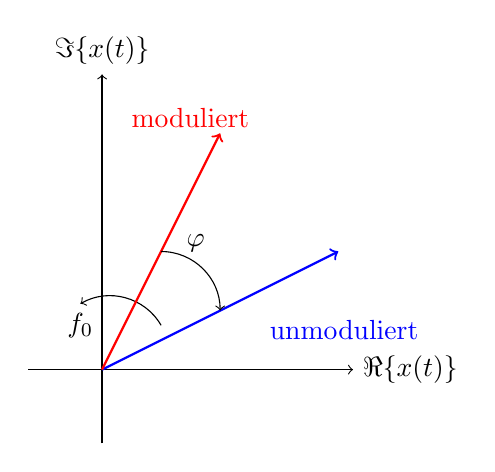
\begin{tikzpicture}[scale=0.75,
        dot/.style={circle,fill=blue,minimum size=3pt,inner sep=0pt,
            outer sep=-1pt},domain=0:4]
\draw[->] (-1.25,0) -- (4.25,0) node[right] {$\Re\lbrace x(t)\rbrace$};
\draw[->] (0,-1.25) -- (0,5) node[above] {$\Im\lbrace x(t)\rbrace$};

\draw[->, color=blue,thick] (0,0) -- (4,2) node[below=10mm, right=-10mm]{\text{unmoduliert}};
\draw[->]  (1,0.75) arc (30:120:1) node[below] {$f_0$};     

\draw[->, color=red,thick] (0,0) -- (2,4) node[above=2mm, left=-5mm]{\text{moduliert}};      
\draw[<-]  (2,1) arc (0:90:1) node[above=1mm, right=2mm] {$\varphi$};    

\end{tikzpicture}
}&
 \parbox{7cm}{
Weitere Eigenschaften der Winkelmodulation ist, dass wenn man eine PM-Modulation integriert eine FM-Modulation erhält. Andersrum eine FM-Modulation differenziert eine PM-Modulation erhält.Den Unterschied zwischen PM und FM erkennt man bei der Variation der Informationsfrequenz $\Omega$. Verdoppelt man $\Omega$, so verdoppelt sich die Bandbreite des PM-Signals entsprechend, da der Abstand der Spektrallinien gerade $\Omega$ beträgt. Da bei der FM-Modulation der Frequenzhub konstant gehalten wird, verdoppelt sich die Bandbreite nicht.
\begin{flalign*}
&\text{FM:} &B_x = 2(\Delta f_0 +F)~ & 			&\Delta \omega = 2 \pi \Delta f_0 \\
&~			&F \ll \Delta f_0~		&			&B_x \approx 2 \Delta f_0	\\
&\text{PM:} &B_x = 2(m+1)F~ & 					&\Omega = 2 \pi F \\
&~			&m \gg 1~		&			&B_x \approx 2mF
\end{flalign*}}
\end{tabular}
\subsection{Bandbreite}
\begin{tabular}{ll} \parbox{8cm}{
Die Bandbreite $B_x$ des modulierten Signalträgers und die Bandbreite $B_s$ des modulierten Primärsignals oder Informationssignals  bestimmen ob es eine schmalbandige oder breitbandige Modulationsart ist. Je Breiter das Band ist, desto störunempfindlicher und desto mehr Daten können übertragen werden.
} & \parbox{3cm}{
\begin{eqnarray*}
\frac{B_x}{B_s} &\lesssim& 2 \quad \text{schmalbandig z.B. AM}\\
\frac{B_x}{B_s} &\gg& 2 \quad \text{breitbandig z.B. FM, PM}
\end{eqnarray*}
} \end{tabular}\\~
\vfill\columnbreak
\subsection{PAM - Pulsamplitudenmodulation}
\begin{tabular}{ll} \parbox{5cm}{
Es gibt diskrete Pegel die definiert sind durch $A_m$, die Adresse des Datums definiert. Die Pulse werden mit einer Bitrate von $R_b = \frac{1}{T_b}$, wobei $T_b$ das Bitintervall ist. Es können pro Übertragungszeitintervall $k$-Bits (Symbole) übertragen werden. $M$ stellt die Menge der möglichen Amplitudenwerte dar, die durch $M = 2^k$ mit $k$-bit langen Symbolblöcken zugeordnet sind. Die festgesetzten Bitrate bei einem  Symbolintervall $T = \frac{k}{R_b} = kT_b$. Wobei $2d$ die Distanz der benachbarten Nachrichten ist.  Alle Signale besitzen verschiedene Energie, die im wesentlichen von $E_g$, der Energie des Pulses $g(t)$ abhängt. \\~
} & \parbox{6cm}{
\setlength\jot{5mm}
\begin{align*}
s_m(t) =& \Re\lbrace A_m \cdot g(t) \cdot e^{j2 \pi f_0 t} \rbrace &~ \text{Zweiseitenband}& \\
=& A_m \cdot g(t) \cdot cos(2 \pi f_0 t)  &~ 0 \leqslant t \leqslant T&\\
A_m =& (2m-1-M)d &~ m=1,2,..,M&
\end{align*}
\begin{eqnarray*}
E_m &=& \int_0^T \vert s_m(t) \vert^2 dt = \underbrace{ \frac{1}{2} }_{\Leftrightarrow \int cos()} A_m^2 \int_0^T g^2(t) dt = \frac{A_m^2}{2} E_g
\end{eqnarray*}}
 \end{tabular}\\~
 \begin{tabular}{ll}
 \parbox{6cm}{
 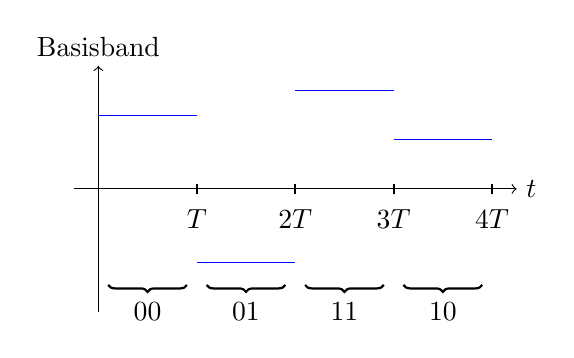
\begin{tikzpicture}[scale=1.25]
\draw[->] (-0.25,0) -- (4.25,0) node[right] {$t$};
\draw[->] (0,-1.25) -- (0,1.25) node[above] {Basisband};

\draw[thick] (1,-1.5pt) -- (1,1.5pt) node[below=2mm] {$T$};
\draw[thick] (2,-1.5pt) -- (2,1.5pt) node[below=2mm] {$2T$}; 
\draw[thick] (3,-1.5pt) -- (3,1.5pt) node[below=2mm] {$3T$}; 
\draw[thick] (4,-1.5pt) -- (4,1.5pt) node[below=2mm] {$4T$}; 

\draw[thick,decoration={brace,mirror,raise=1cm}, decorate] (0.1,-5pt) -- (0.9,-5pt);
\node (note1) at (0.5,-1.25)  {00};
\draw[thick,decoration={brace,mirror,raise=1cm}, decorate] (1.1,-5pt) -- (1.9,-5pt);
\node (note1) at (1.5,-1.25)  {01};
\draw[thick,decoration={brace,mirror,raise=1cm}, decorate] (2.1,-5pt) -- (2.9,-5pt);
\node (note1) at (2.5,-1.25)  {11};
\draw[thick,decoration={brace,mirror,raise=1cm}, decorate] (3.1,-5pt) -- (3.9,-5pt);
\node (note1) at (3.5,-1.25)  {10};

\draw[color=blue] (0,0.75) -- (1,0.75);
\draw[color=blue] (1,-0.75) -- (2,-0.75);
\draw[color=blue] (2,1) -- (3,1);
\draw[color=blue] (3,0.5) -- (4,0.5);

\end{tikzpicture}\\~
}&
 \parbox{7cm}{
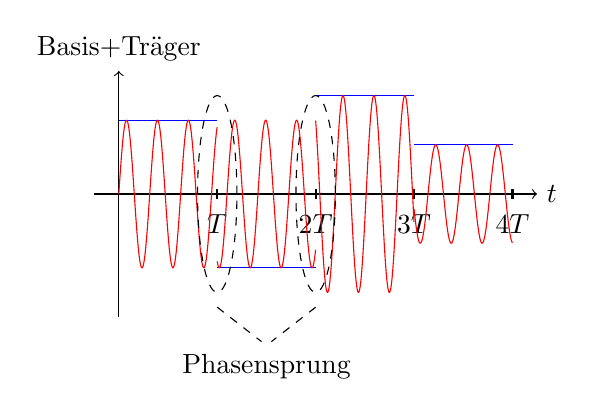
\begin{tikzpicture}[scale=1.25]
\draw[->] (-0.25,0) -- (4.25,0) node[right] {$t$};
\draw[->] (0,-1.25) -- (0,1.25) node[above] {Basis+Träger};

\draw[thick] (1,-1.5pt) -- (1,1.5pt) node[below=2mm] {$T$};
\draw[thick] (2,-1.5pt) -- (2,1.5pt) node[below=2mm] {$2T$}; 
\draw[thick] (3,-1.5pt) -- (3,1.5pt) node[below=2mm] {$3T$}; 
\draw[thick] (4,-1.5pt) -- (4,1.5pt) node[below=2mm] {$4T$}; 

\draw[color=blue] (0,0.75) -- (1,0.75);
\draw[color=blue] (1,-0.75) -- (2,-0.75);
\draw[color=blue] (2,1) -- (3,1);
\draw[color=blue] (3,0.5) -- (4,0.5);

\draw[color=red, domain=0:1, samples=200]   plot(\x,{(0.75*(sin(20*\x r))}); 
\draw[color=red, domain=1:2, samples=200]   plot(\x,{(-0.75*(sin(20*\x r))}); 
\draw[color=red, domain=2:3, samples=200]   plot(\x,{(1*(sin(20*\x r))}); 
\draw[color=red, domain=3:4, samples=200]   plot(\x,{(0.5*(sin(20*\x r))}); 

\draw[color=black, dashed] (1,0) ellipse (2mm and 1cm);
\draw[color=black, dashed] (2,0) ellipse (2mm and 1cm);

\draw[color=black, dashed] (2,-1.15) -- (1.55,-1.5);
\draw[color=black, dashed] (1,-1.15) -- (1.45,-1.5);

\node (note1) at (1.5,-1.75)  {Phasensprung};
\end{tikzpicture}\\~ }
 \end{tabular}\\~
Jedes der Symbole (00, 01, 11 ,10) wird in einem Symbolintervall $kT_b$ gesendet. Je geringer die Distanz zwischen den Signalen ist, desto schwerer ist es diese zu detektieren. Die minimale Euklidische Distanz zwischen zwei benachbarten Signalpunkten ist:
 \begin{eqnarray*}
 d^{(e)}_{mn} = \sqrt{(s_m - s_n)^2} &=& \sqrt{\frac{E_g}{2}} \vert A_m - A_n \vert = d \sqrt{2 E_g} \vert m-n \vert
 \end{eqnarray*}
Somit ist das PAM-Signal ein Zweiseitenband-AM-Signal und benötigt wie im Fall der analogen Modulation die doppelte Bandbreite (schmalbandiges Verfahren). Im wesentlichen sind PAM-Signale eindimensional, sie können dennoch auch zweidimensional sein, diese werden durch orthogonale Signale mit identischer Energie $A^2T$ und somit die euklidische Distanz $d_12 = \sqrt{2E_g}$.\\\vspace{6pt}
\textbf{Beispiel:} \quad M-äre Modulation mit 5-Bit Symbolblöcken. Welche Art?\\\vspace{6pt}
 \begin{tabular}{ll}
 \parbox{4cm}{
$\underbrace{01001}~ \underbrace{01101}~\underbrace{11101}~\underbrace{10100}$ }&
 \parbox{7cm}{
 Unterteilung von $k$-Bits (hier 5) in Symbole. Jedes Symbol ist einzigartig für jede mögliche Bitkombination. Es werden $2^k$ Symbole benötigt.
 }
 \end{tabular}\\\vspace{6pt}
Wenn eine Übertragung mit 10kBaud $\frac{R}{K}$ (Symbole pro Sekunde) stattfindet, wäre die Bitübertragungsrate  $R = \frac{R}{K} \cdot K$ 50kBit.\\~\vspace{2pt}\\~
\subsection{PSK - Phase-Shift-Keying}
\begin{tabular}{ll} \parbox{3cm}{
Es gibt diskrete Phasen des Signals die einem Symbol zugeordnet werden. Eine PSK mit $M=2$ ist eine PAM. Eine PSK-Modulation mit $M=2$ wird auch als Binary-Phase-Shift Keying (\textbf{BPSK}), $M=4$ QPSK und $M=8$ als Octal PSK bezeichnet. Bei zu vielen PSK ist es schwer das Signal zu detektieren. Für alle PSK-Signale gilt die gleiche Energie.
} & \parbox{8cm}{
\setlength\jot{5mm}
\begin{align*}
s_m(t) =& \Re\lbrace g(t) e^{j2 \pi \frac{(m-1)}{M}} e^{j2 \pi f_c t} \rbrace &~ m = 1, 2,...,M& \\
=&  g(t) \cdot cos\left( 2 \pi f_c t + \frac{2\pi (m-1)}{M}\right)   &~ ~&\\
=&  g(t) cos\left( \frac{2 \pi (m-1)}{M}\right) cos(2 \pi f_c t)- g(t) sin\left( \frac{2 \pi (m-1)}{M}\right) sin(2 \pi f_c t)  &~ ~&\
\end{align*}
\begin{eqnarray*}
E_m &=& \int_0^T \vert s_m(t) \vert^2 dt = \underbrace{ \frac{1}{2} }_{\int cos()}\int g^2(t) dt = \frac{E_g}{2}
\end{eqnarray*}}
 \end{tabular}\\~
\vspace{6pt}
Offensichtlich kann diese Modulationsart durch zwei othonormale Basen dargestellt werden:
\begin{align*}
&s_m(t) = s_{m1} \cdot f_1(t) + s_{m2} \cdot f_2(t) ~&\\
&f_1(t) = \sqrt{\frac{2}{E_g}} g(t) cos(2 \pi f_c t) &f_2(t) = -\sqrt{\frac{2}{E_g}} g(t) sin(2 \pi f_c t)
\end{align*}
 \begin{tabular}{ll}
 \parbox{6cm}{
 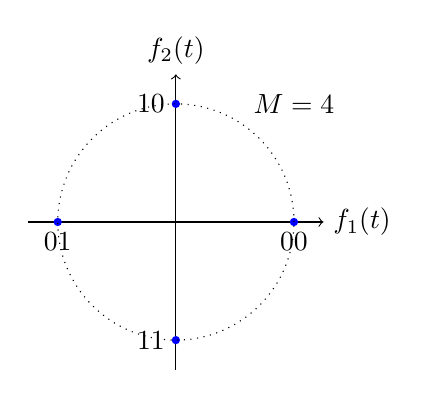
\begin{tikzpicture}[scale=1.5, dot/.style={circle,fill=blue,minimum size=3pt,inner sep=0pt,outer sep=-1pt}]
\draw[->] (-1.25,0) -- (1.25,0) node[right] {$f_1(t)$};
\draw[->] (0,-1.25) -- (0,1.25) node[above] {$f_2(t)$};

\node[dot,label=below:$00$] at (1,0)(int1) {};
\node[dot,label=below:$01$] at (-1,0)(int1) {}; 
\node[dot,label=left:$10$] at (0,1)(int1) {}; 
\node[dot,label=left:$11$] at (0,-1)(int1) {}; 
\node (note1) at (1,1)  {$M=4$};
\draw[dotted]  (1,0) arc (0:360:1);

\end{tikzpicture}\\~
}&
 \parbox{5cm}{
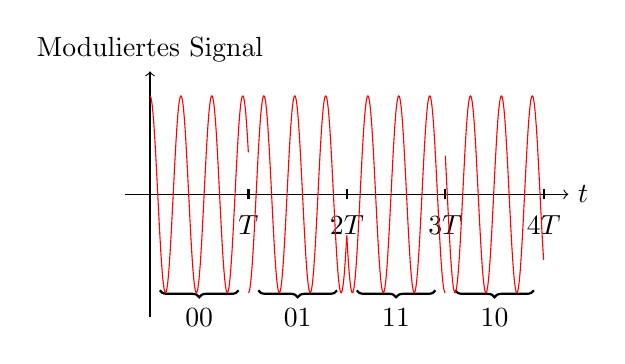
\begin{tikzpicture}[scale=1.25]
\draw[->] (-0.25,0) -- (4.25,0) node[right] {$t$};
\draw[->] (0,-1.25) -- (0,1.25) node[above] {Moduliertes Signal};

\draw[thick] (1,-1.5pt) -- (1,1.5pt) node[below=2mm] {$T$};
\draw[thick] (2,-1.5pt) -- (2,1.5pt) node[below=2mm] {$2T$}; 
\draw[thick] (3,-1.5pt) -- (3,1.5pt) node[below=2mm] {$3T$}; 
\draw[thick] (4,-1.5pt) -- (4,1.5pt) node[below=2mm] {$4T$}; 

\draw[thick,decoration={brace,mirror,raise=1cm}, decorate] (0.1,-5pt) -- (0.9,-5pt);
\node (note1) at (0.5,-1.25)  {00}; 
\draw[thick,decoration={brace,mirror,raise=1cm}, decorate] (1.1,-5pt) -- (1.9,-5pt);
\node (note1) at (1.5,-1.25)  {01}; 
\draw[thick,decoration={brace,mirror,raise=1cm}, decorate] (2.1,-5pt) -- (2.9,-5pt);
\node (note1) at (2.5,-1.25)  {11};
\draw[thick,decoration={brace,mirror,raise=1cm}, decorate] (3.1,-5pt) -- (3.9,-5pt);
\node (note1) at (3.5,-1.25)  {10}; 

\draw[color=red, domain=0:1, samples=200]   plot(\x,{(cos((20*\x) r)}); 
\draw[color=red, domain=1:2, samples=200]   plot(\x,{(cos((20*\x+2) r)}); 
\draw[color=red, domain=2:3, samples=200]   plot(\x,{(cos((20*\x+6) r)}); 
\draw[color=red, domain=3:4, samples=200]   plot(\x,{(cos((20*\x+4) r)}); 
\end{tikzpicture}\\~ }
 \end{tabular}\\
Diese Signalform kann in einen sogenannten \textbf{Q}uadraturanteil ($Q = sin(\Omega)$) und in einen \textbf{I}nphasenanteil ($I = cos(\Omega)$) aufgeteilt werden. Für die Amplitude des Signals gilt $A^2 = I^2 + Q^2$. Die euklidische Distanz zwischen zwei PSK-Signalen $s_m(t)$ und $s_n(t)$ kann ausgedrückt werden durch:
\begin{align*}
&I^2 = \left[cos\left(\frac{2 \pi}{M}(m-1) \right)-cos\left(\frac{2 \pi}{M}(n-1) \right)  \right]  &Q^2 = \left[sin\left(\frac{2 \pi}{M}(m-1) \right)-sin\left(\frac{2 \pi}{M}(n-1) \right)  \right] \\ 
&\left( d^{e}_{mn} \right)^2  = \Vert s_m - s_n \Vert^2 = \frac{E_g}{2}(I^2 + Q^2) &\Rightarrow \left( d^{e}_{mn} \right)^2  = \sqrt{E_g \left[1-cos\left(\frac{2 \pi}{M}(m-n) \right)  \right] } \\
&\text{min. euklidische Distanz:} &d^e_{min} = \Vert s_m - s_n \Vert = \sqrt{E_g \left[1-cos\left(\frac{2 \pi}{M}) \right)  \right] }
\end{align*}
\textbf{Beispiel:} \quad M-äre Modulation mit 5-Bit Symbolblöcken. Welche Art?\\\vspace{6pt}
 \begin{tabular}{ll}
 \parbox{4cm}{
$\underbrace{01001}~ \underbrace{01101}~\underbrace{11101}~\underbrace{10100}$ }&
 \parbox{7cm}{
 Unterteilung von $k$-Bits (hier 5) in Symbole. Jedes Symbol ist einzigartig für jede mögliche Bitkombination. Es werden $2^k$ Symbole benötigt.
 }
 \end{tabular}\\\vspace{6pt}
\subsection{QAM - Quadraturamplitudenmodulation}
\begin{tabular}{ll} \parbox{4.5cm}{
Eine QAM kann als $M_1$-stufige PAM und als $M_2$-stufige PSK dargestellt werden. Sogenannte zweidimensinale Bandpasssignale. Wobei $A_{mc}$ und $A_{ms}$ die Informationstragenden Signalamplituden der Quadraturträger und $g(t)$ eine Pulsform darstellen. Es werden wieder $k$-Bit-Symbole der Informationssequenz $a_n$ auf zwei in Quadratur befindliche Trägersignale $cos(2 \pi f_c t)$ und $sin(2 \pi f_c t)$ moduliert.\\} & \parbox{5.5cm}{
\setlength\jot{5mm}
\begin{align*}
s_m(t) =& \Re\lbrace \left[ A_{mc} + jA_{ms} \right] e^{j2 \pi f_c t} g(t) \rbrace &~ m = 1, 2,...,M& \\
=&  A_{mc} g(t) cos(2 \pi f_ct) - A_{ms} g(t) sin(2 \pi f_ct)   &~ ~&\\
\end{align*}}
 \end{tabular}\\~
\vspace{6pt}
Offensichtlich kann diese Modulationsart durch zwei othonormale Basen dargestellt werden:
\begin{align*}
&s_m(t) = s_{m1} \cdot f_1(t) + s_{m2} \cdot f_2(t) &s_{m1}(t) = <s_m(t), f_1(t)> = \int^T_0 s_m(t) f_1^*(t) dt\\
&s_m(t) = \left[ A_{mc}\sqrt{\frac{E_g}{2}} \quad   A_{ms}\sqrt{\frac{E_g}{2}}\right] &~
\end{align*}
 \begin{tabular}{ll}
 \parbox{5cm}{
 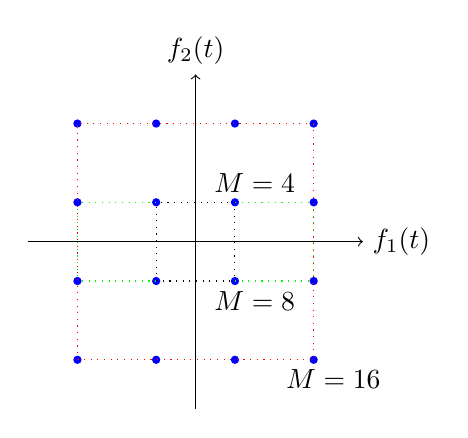
\begin{tikzpicture}[scale=0.5, dot/.style={circle,fill=blue,minimum size=3pt,inner sep=0pt,outer sep=-1pt}]
\draw[->] (-4.25,0) -- (4.25,0) node[right] {$f_1(t)$};
\draw[->] (0,-4.25) -- (0,4.25) node[above] {$f_2(t)$};

\node[dot] at (1,1)(int1) {};
\node[dot] at (1,-1)(int1) {};
\node[dot] at (-1,1)(int1) {};
\node[dot] at (-1,-1)(int1) {};

\draw[dotted] (1,1) -- (1,-1);
\draw[dotted] (1,1) -- (-1,1);
\draw[dotted] (-1,-1) -- (1,-1);
\draw[dotted] (-1,-1) -- (-1,1);

\node (note1) at (1.5,1.5)  {$M=4$};

\node[dot] at (3,3)(int1) {};
\node[dot] at (3,-3)(int1) {};
\node[dot] at (-3,3)(int1) {};
\node[dot] at (-3,-3)(int1) {};

\draw[dotted, color=green] (1,-1) -- (3,-1);
\draw[dotted, color=green] (-1,-1) -- (-3,-1);
\draw[dotted, color=green] (1,1) -- (3,1);
\draw[dotted, color=green] (-1,1) -- (-3,1);
\draw[dotted, color=green] (3,1) -- (3,-1);
\draw[dotted, color=green] (-3,1) -- (-3,-1);

\node (note1) at (1.5,-1.5)  {$M=8$};

\node[dot] at (3,1)(int1) {};
\node[dot] at (3,-1)(int1) {};
\node[dot] at (-3,1)(int1) {};
\node[dot] at (-3,-1)(int1) {};

\node[dot] at (1,3)(int1) {};
\node[dot] at (1,-3)(int1) {};
\node[dot] at (-1,3)(int1) {};
\node[dot] at (-1,-3)(int1) {};

\draw[dotted, color=red] (3,3) -- (3,-3);
\draw[dotted, color=red] (3,3) -- (-3,3);
\draw[dotted, color=red] (-3,-3) -- (3,-3);
\draw[dotted, color=red] (-3,-3) -- (-3,3);

\node (note1) at (3.5,-3.5)  {$M=16$};

\end{tikzpicture}\\~
}&
 \parbox{5cm}{
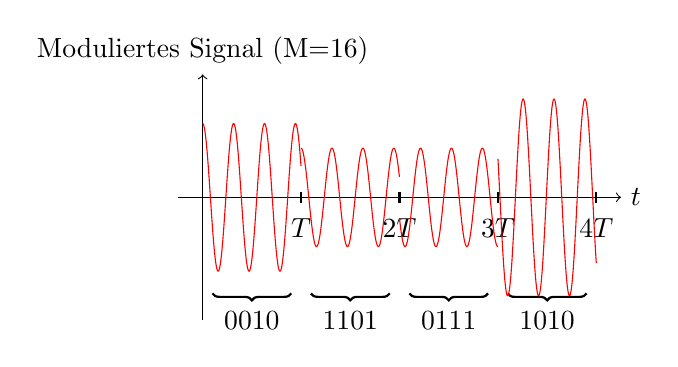
\begin{tikzpicture}[scale=1.25]
\draw[->] (-0.25,0) -- (4.25,0) node[right] {$t$};
\draw[->] (0,-1.25) -- (0,1.25) node[above] {Moduliertes Signal (M=16)};

\draw[thick] (1,-1.5pt) -- (1,1.5pt) node[below=2mm] {$T$};
\draw[thick] (2,-1.5pt) -- (2,1.5pt) node[below=2mm] {$2T$}; 
\draw[thick] (3,-1.5pt) -- (3,1.5pt) node[below=2mm] {$3T$}; 
\draw[thick] (4,-1.5pt) -- (4,1.5pt) node[below=2mm] {$4T$}; 

\draw[thick,decoration={brace,mirror,raise=1cm}, decorate] (0.1,-5pt) -- (0.9,-5pt);
\node (note1) at (0.5,-1.25)  {0010}; 
\draw[thick,decoration={brace,mirror,raise=1cm}, decorate] (1.1,-5pt) -- (1.9,-5pt);
\node (note1) at (1.5,-1.25)  {1101}; 
\draw[thick,decoration={brace,mirror,raise=1cm}, decorate] (2.1,-5pt) -- (2.9,-5pt); 
\node (note1) at (2.5,-1.25)  {0111}; 
\draw[thick,decoration={brace,mirror,raise=1cm}, decorate] (3.1,-5pt) -- (3.9,-5pt);
\node (note1) at (3.5,-1.25)  {1010};

\draw[color=red, domain=0:1, samples=200]   plot(\x,{0.75*(cos((20*\x) r)}); 
\draw[color=red, domain=1:2, samples=200]   plot(\x,{(-0.5)*(cos((20*\x+2) r)}); 
\draw[color=red, domain=2:3, samples=200]   plot(\x,{0.5*(cos((20*\x+6) r)}); 
\draw[color=red, domain=3:4, samples=200]   plot(\x,{(cos((20*\x+4) r)}); 
\end{tikzpicture}\\~ }
 \end{tabular}\\
Diese Signalform kann in einen sogenannten \textbf{Q}uadraturanteil ($Q = sin(\Omega)$) und in einen \textbf{I}nphasenanteil ($I = cos(\Omega)$) aufgeteilt werden. Weiteres siehe PSK. Bei der Betrachtung einer rechtwinkligen Raumkonstellation (siehe Diagramm oben links) müssen die Punkte aller 2-er Potenzen darstellen, um die Bits zu Interpätieren. Eine Quadratur der Konstellationspunkte hat eine Verdopplung der Signalmenge zur Folge. Der Abstand zweier benachbarter Signalpunkte ist immer identisch!
\begin{align*}
&\text{min. euklidische Distanz:} &d^e_{min} = \Vert s_m - s_n \Vert = \sqrt{\frac{E_g}{2} \left[(A_{mc}+A_{nc})^2 +  (A_{ms}-A_{ns})^2 \right] }
\end{align*}
\textbf{Beispiel:} \quad M-äre Modulation mit 5-Bit Symbolblöcken. Welche Art?\\\vspace{6pt}
 \begin{tabular}{ll}
 \parbox{4cm}{
$\underbrace{01001}~ \underbrace{01101}~\underbrace{11101}~\underbrace{10100}$ }&
 \parbox{9cm}{
 Unterteilung von $k$-Bits (hier 5) in Symbole. Jedes Symbol ist einzigartig für jede mögliche Bitkombination. Es werden $2^5 = 32$ Symbole benötigt. Es kann somit eine 32-QAM verwendet werden. Es sind größere QAMs möglich. Es wird nur jedes zweite Signal verwendet, somit ist der Signal-Rauschabstand (SNR) geringer.
 }
 \end{tabular}\\\vspace{6pt}
\subsection{Orthogonale Entwicklung von Signalen \& FSK}
Bei der orthogonalen Entwicklung von Signalen wird durch Projektion der Signale auf geeignete Basen eine Signalraum der Dimension M geschaffen. Jedes der Signale kann eine Information enthalten. Eine Information entspricht einem Symbol.\\
\begin{tabular}{lll}
 \addtolength{\jot}{2mm}
 \parbox{3cm}{
\begin{tikzpicture}[scale=0.4] 
\draw[->] (-0.25,0) -- (4,0) node[right] {$t$};
\draw[->] (0,-0.25) -- (0,1.5) node[above] {$f_1(t)$};
	
\draw[dashed, color=red] (0,0) -- (0,1);
\draw[color=red] (0,1) -- (1,1);
\draw[dashed, color=red] (1,0) -- (1,1);
\end{tikzpicture}
\begin{tikzpicture}[scale=0.4] 
\draw[->] (-0.25,0) -- (4,0) node[right] {$t$};
\draw[->] (0,-0.25) -- (0,1.5) node[above] {$f_2(t)$};
	
\draw[dashed, color=red] (1,0) -- (1,1);
\draw[color=red] (1,1) -- (2,1);
\draw[dashed, color=red] (2,0) -- (2,1);
\end{tikzpicture} 
\begin{tikzpicture}[scale=0.4] 
\draw[->] (-0.25,0) -- (4,0) node[right] {$t$};
\draw[->] (0,-0.25) -- (0,1.5) node[above] {$f_3(t)$};
	
\draw[dashed, color=red] (2,0) -- (2,1);
\draw[color=red] (2,1) -- (3,1);
\draw[dashed, color=red] (3,0) -- (3,1);
\end{tikzpicture} \\~  
 }
 &
 \parbox{4cm}{
 \begin{tikzpicture}[scale=0.55,  dot/.style={circle,fill=red,minimum size=3pt,inner sep=0pt, outer sep=-1pt}]
\draw[->, thick] (0,0,0) -- (3,0,0) node[anchor=north east, right=1mm]{$f_1$};
\draw[dashed, thick] (0,0,0) -- (-3,0,0);
\draw[->, thick] (0,0,0) -- (0,3,0) node[anchor=north west, left=1mm]{$f_2$};
\draw[dashed, thick] (0,0,0) -- (0,-3,0);
\draw[->, thick] (0,0,0) -- (0,0,3) node[anchor=south, right=1mm, below=1mm]{$f_3$};
\draw[dashed, thick] (0,0,0) -- (0,0,-3);

\draw[color=blue] (-2,0,0) -- (2,0,0);
\draw[color=blue] (-2,0,-2) -- (2,0,-2);
\draw[color=blue] (-2,-2,0) -- (2,-2,0);
\draw[color=blue] (-2,-2,-2) -- (2,-2,-2);
\draw[color=blue] (0,2,0) -- (2,2,0);
\draw[color=blue] (0,2,-2) -- (2,2,-2);

\draw[color=blue] (2,0,0) -- (2,0,-2);
\draw[color=blue] (2,-2,0) -- (2,-2,-2);
\draw[color=blue] (2,2,0) -- (2,2,-2);
\draw[color=blue] (0,2,0) -- (0,2,-2);
\draw[color=blue] (0,0,0) -- (0,0,-2);
\draw[color=blue] (0,-2,0) -- (0,-2,-2);
\draw[color=blue] (-2,0,0) -- (-2,0,-2);
\draw[color=blue] (-2,-2,0) -- (-2,-2,-2);

\draw[color=blue] (-2,0,0) -- (-2,-2,0);
\draw[color=blue] (-2,0,-2) -- (-2,-2,-2);
\draw[color=blue] (0,2,0) -- (0,-2,0);
\draw[color=blue] (0,2,-2) -- (0,-2,-2);
\draw[color=blue] (2,2,0) -- (2,-2,0);
\draw[color=blue] (2,2,-2) -- (2,-2,-2);

\node[dot] at (2,2,0) {$s_1$}; 
\node[dot] at (2,2,-2) {$s_2$}; 
\node[dot] at (2,-2,0) {$s_3$}; 
\node[dot] at (-2,0,-2) {$s_4$}; 
\end{tikzpicture}}
 &
 \parbox{4cm}{\begin{tikzpicture}[scale=0.3] 
\draw[->] (-0.25,0) -- (4,0) node[right] {$t$};
\draw[->] (0,-1.25) -- (0,1.25) node[above] {$s_1(t)$};
	
\draw[dashed, color=red] (0,0) -- (0,1);
\draw[color=red] (0,1) -- (3,1);
\draw[dashed, color=red] (3,0) -- (3,1);
\end{tikzpicture}
\begin{tikzpicture}[scale=0.3] 
\draw[->] (-0.25,0) -- (4,0) node[right] {$t$};
\draw[->] (0,-1.25) -- (0,1.25) node[above] {$s_2(t)$};
	
\draw[dashed, color=red] (0,0) -- (0,1);
\draw[color=red] (0,1) -- (2,1);
\draw[dashed, color=red] (2,-1) -- (2,1);
\draw[color=red] (2,-1) -- (3,-1);
\draw[dashed, color=red] (3,-1) -- (3,0);
\end{tikzpicture} 
\begin{tikzpicture}[scale=0.3] 
\draw[->] (-0.25,0) -- (4,0) node[right] {$t$};
\draw[->] (0,-1.25) -- (0,1.25) node[above] {$s_3(t)$};
	
\draw[dashed, color=red] (0,0) -- (0,1);
\draw[color=red] (0,1) -- (1,1);
\draw[dashed, color=red] (1,-1) -- (1,1);
\draw[color=red] (1,-1) -- (2,-1);
\draw[dashed, color=red] (2,-1) -- (2,0);
\end{tikzpicture} \\~}
\end{tabular}\\~
\vspace{6pt}
\begin{tabular}{ll}
 \addtolength{\jot}{2mm}
 \parbox{5cm}{Wenn das Skalarprodukt zweier Signale null ergibt, dann sind diese Signale zueinander orthogonal. Wenn sie zudem noch die Norm 1 besitzen, sind sie orthonormal. Es wird immer die Energie des Signals normiert! Um Signale entsprechend zu entwickeln muss eine orthonormale Basis (siehe Plot $f_1$, $f_2$, $f_3$) gebildet werden. }
 &
 \parbox{7.5cm}{
 \begin{eqnarray*}
 < x_1(t) , x_2(t)> &=& \int x_1(t) \cdot x^*_2(t) dt\\
 \Vert x(t) \Vert  &=& \sqrt{ < x(t) , x(t)>} = \sqrt{\int \vert x(t) \vert^2 dt}\\
 E_k(t) &=& \Vert s_{kn} \Vert^2 
 \end{eqnarray*} (Orthogonal bedeutet das die Vektoren lin. unabh. sind, aber nicht andersrum!)}
\end{tabular}\\~

\begin{tabular}{ll}
 \addtolength{\jot}{2mm}
 \parbox{7.5cm}{
 \begin{eqnarray*}
 s(t) &=& \sum_{i \in \mathbb{Z}} s_i f_i(t)\\
g_1(t) &=& \frac{s_1(t)}{\Vert s_1(t) \Vert}\\
g_2(t) &=& \frac{s_2(t)-<s_2(t),f_1(t)> \cdot f_1(t)}{\Vert s_2(t)-<s_2(t),f_1(t)> \cdot f_1(t) \Vert}\\
&~& \\
f_k(t) &=&  \frac{s_k(t) - \sum_{i=1}^{k-1} <s_k(t), f_i(t)> \cdot f_i(t)}{\sqrt{\int \vert s_k(t) - \sum_{i=1}^{k-1} <s_k(t), f_i(t)> \cdot f_i(t) \vert^2 dt}}
 \end{eqnarray*}}&
 \parbox{5cm}{Durch Projektion der einzelnen Signale auf eine Basis kann das Signal beschrieben werden. Wenn die Energie des Restfehlers ($E_p = \Vert s(t) - \hat{s}(t) \Vert = 0$) null für jedes Signal ergibt, dann ist die Basis vollständig beschrieben. Ein  \textbf{einfaches Vorgehen} ist Nebenstehend mit den Basen $g_1(t)$ und $g_2(t)$ gezeigt. Hierbei wird das Signal $s_1(t)$ als erste normierte Basis verwendet. Danach wird die Komponenten von $f_1(t)$ von dem zweiten Signal $s_2(t)$ abgezogen und normiert. Allgemein kann dies auch mit der Formel $f_k(t)$ gezeigt werden. Hier muss drauf geachtet werden das die Signale $s_k(t)$ alle linear unabhängig sind. Lin. Unab. prüfen:
$\alpha_1 s_1(t) + \alpha_2 s_2(t) + ... = 0 \Rightarrow \alpha_1 = \alpha_2 = ... = 0$}
\end{tabular}
\begin{tabular}{ll}
 \addtolength{\jot}{2mm}
 \parbox{4cm}{
 \begin{tikzpicture}[scale=0.6] 
\draw[->] (-0.25,0) -- (3.75,0) node[right] {$f$};
\draw[->] (0,-0.25) -- (0,3.75) node[above] {$t$};
	
\draw[dashed] (0,1) -- (3,1);
\draw[dashed] (0,2) -- (3,2);
\draw[dashed] (0,3) -- (3,3);
\draw[dashed] (1,0) -- (1,3);
\draw[dashed] (2,0) -- (2,3);
\draw[dashed] (3,0) -- (3,3);

\draw[thick] (1,-1.5pt) -- (1,1.5pt) node[below=2mm] {$T$};
\draw[thick] (2,-1.5pt) -- (2,1.5pt) node[below=2mm] {$2T$};
\draw[thick] (3,-1.5pt) -- (3,1.5pt) node[below=2mm] {$3T$};
\draw[thick] (-1.5pt,1) -- (1.5pt,1) node[left=1mm] {$f_0+\vartriangle f$};  
\draw[thick] (-1.5pt,2) -- (1.5pt,2) node[left=1mm] {$f_0+2\vartriangle f$};  
\draw[thick] (-1.5pt,3) -- (1.5pt,3) node[left=1mm] {$f_0+3\vartriangle f$};  
\end{tikzpicture}}&
 \parbox{9cm}{Eine \textbf{mehrdimensionale Signalisierung} erlaubt das übertragen mehrerer Signale auf einmal (z.B. bei PAM-Signalen) .Es werden pro Zeiteinheit T N-Signale gleichzeitig übertragen (\textbf{Frequency-Shift-Keying}. Es kann eine Unterteilung in Zeit und Frequenzbereich vorgenommen werden. Hierdurch werden sogenannte Kurzzeitspektren erzeugt, sprich zu einer gewissen Zeit gibt es ein Signal (ähnlich Notenblatt). Dieses Vorgehen wird bei z.B. 12 Zeit und Frequenzschlitzen um einen 24-dimensionalen Signalvektor zu übertragen, 4-QAM genannt (2bit).}
\end{tabular}\\~
\vfill\columnbreak
\subsection{Kreuzkorrelation}
\begin{tabular}{ll}
 \addtolength{\jot}{2mm}
 \parbox{7.5cm}{Die Kreuzkorrelation beschreibt die Ähnlichkeit zweier Signale. Durch die Normierung wird das Ähnlichkeitsmaß $\vert \delta_{km} \vert \in [0,1]$ begrenzt. Das Innere Produkt erzeugt die Projektion auf den Vektor. Der Kreuzkorrelationskoeffizient ist eine komplexe Zahl im Einheitskreis. Wenn $\delta_{km} = 1$, dann sich die Signale vielfache voneinander. Wenn die Signale reellwertig sind, dann beschreibt $\delta_{km}$ den Kosinus des eingeschlossenen Winkels (nur Reelle Achse). Ist das Signal komplexwertig, liegt das Signal im gesamten Einheitskreis. Bei $\delta_{km} = 0$ sind die Signale orthogonal zueinander. Bei $\delta_{km} = 1$, ist die Phasenverschiebung $180^{\circ}$.
}&
 \parbox{4cm}{
  \addtolength{\jot}{2mm}
 \begin{equation*}
\delta_{km} = \frac{< s_{lk}(t) , s_{lm}(t) >}{\Vert s_{lk}(t) \Vert \cdot \Vert s_{lm}(t) \Vert}
 \end{equation*}
 \begin{eqnarray*}
 &\text{für FSK:} \\
\delta_{km} &= \dfrac{\frac{2E}{T}}{2E} \int^T_0 e^{j2 \pi (k-m) \Delta ft} dt \\
&= \dfrac{sin(nT(k-m)\Delta f}{nT(k-m)\Delta f} e^{j2 \pi (k-m) \Delta ft} dt
 \end{eqnarray*}
 }
\end{tabular}\\~
\subsection{Simplex-Signale}
\begin{tabular}{ll}
 \addtolength{\jot}{2mm}
 \parbox{10cm}{Um die Energie der Signale geringer zu bekommen, muss der Nullpunkt der Signale verschoben werden und zwar genau in den Mittelwert der orthogonalen Signale. Die Orthogonalität geht durch das verschieben des Nullpunkts verloren, aber die Energie wird geringer und die Distanz zwischen den Signalen bleibt gleich. Durch diese Operation schrumpft die Dimension des Signalraums um 1 (z.B. von 3 auf 2, usw...).
}&
 \parbox{4cm}{
 \begin{equation*}
\bar{s} = \frac{1}{M} \cdot \sum_{m=1}^M s_m 
 \end{equation*}
 }
\end{tabular}\\~
\begin{tabular}{ll}
 \addtolength{\jot}{2mm}
 \parbox{5cm}{
 \begin{tikzpicture}[scale=0.6] 
\draw[->] (-0.25,0) -- (4.5,0) node[right] {$f_1$};
\draw[->] (0,-0.25) -- (0,4.5) node[above] {$f_2$};
	
\draw[thick] (4,-1.5pt) -- (4,1.5pt) node[below=2mm] {$s_1$};  
\draw[thick] (-1.5pt,4) -- (1.5pt,4) node[left=1mm] {$s_2$};  

\draw[->, color=red] (0,0) -- (0,4);  
\draw[->, color=red] (0,0) -- (4,0);

\draw[thick,decoration={brace,raise=0.5cm}, decorate] (0,4) -- (4,0);
\node (note1) at (2.75,3.25)  {$\sqrt{2E}$}; 
\draw[color=black] (0,4) -- (4,0);   
\draw[->, color=blue] (0,0) -- (2,2)node[below=2mm] {$\bar{s}$};   

\end{tikzpicture}
}&
 \parbox{8cm}{
  \addtolength{\jot}{2mm}
 \begin{eqnarray*}
 \displaystyle
 \acute{E_s} &= \int^T_0 \vert \acute{s}_m(t)\vert^2 dt ) \left( 1- \frac{1}{M} \right) E_s \\
 \acute{s_m}(t) &= s_m - \frac{1}{M} \sum^M_{k=1}s_k
\end{eqnarray*}  
 Die Energie jedes der orthogonalen Signale ist im Simplexsignalsatz geringer als im othogonalen Signalsatz. Simplexsignale haben eine negative Korrelation, die für alle Signalpaar gleich ist. Die Distanz zwischen zwei Signalpunkten beträgt $\sqrt{2E}$. Die geometrische Darstellung eines Satzes von M Simplexsignalen erhält man, indem der Durchschnittssignalvektor $\bar{s}$ von dem Satz othogoinaler Signale subtrahiert.
 }
\end{tabular}\\~
\subsection{Signale auf Basis binärer Codes}
\begin{tabular}{ll}
 \addtolength{\jot}{2mm}
 \parbox{5cm}{Die Signale bestehen aus M-Signalen $(m = 1,2,3...,M)$ die binär codiert worden sind, wobei $c_{mj} = 0$ oder $c_{mj} = 1$ für alle $m,j$. Jede Komponente kann mittels BPSK-Signal dargestellt werden. Es existieren somit $2^k$ mögliche Signale, diese können in einem N-Dimensionalen Raum dargestellt werden. Jedes Signal hat die gleiche Energie $E$ und die Kreuzkorrelation der Signale hängt von der Selekttion der Signalmenge M ab.
}&
 \parbox{8cm}{
 \begin{eqnarray*}
c_m &= \left[ c_{m1}, c_{m2}, c_{m3}, ... , c_{mN} \right] \\
~&\\
c_{mj} = 0 &\Rightarrow s_{mj}(t) = \sqrt{\dfrac{2E}{T_e}} \cdot cos (2\pi f_c t)\\
~&\\
c_{mj} = 1 &\Rightarrow s_{mj}(t) = - \sqrt{\dfrac{2E}{T_e}} \cdot cos (2\pi f_c t)\\
~&\\
d &= 2 \sqrt{\dfrac{E_s}{N}}
 \end{eqnarray*}
 }
\end{tabular}\\~
\vfill\columnbreak
